% !TeX root = ../main.tex

\xchapter{模拟器的设计与实现}{Simulator Design and Implementation}

\xsection{问题定义与设计目标}{Problem Definition and Design Goals}\label{sec:c3_problem}

\xsubsection{问题定义}{Problem Definition}\label{subsec:c3_problem}

本研究关注的问题是：在多核神经网络芯片尚未流片或仅有部分硬件原型的早期阶段，如何为体系结构师与系统软件开发者提供一个可信、可控、可迭代的周期级评估手段。该手段应在统一框架下回答以下问题：在给定映射、给定核内规模、给定 NoC 拓扑与给定 DRAM 配置下，端到端推理需要多少周期，瓶颈在哪，调整哪一项硬件参数能带来最大收益。该问题具有三重耦合，即负载侧的算子结构与映射策略、核间通信的拓扑与拥塞、片外存储的带宽与时序。三者中任一项的变化都会经由数据依赖与时序推进改变端到端结果，因此评估手段必须能够把这三层在同一时间轴上协同推进。

现有方案在不同侧面给出了部分答案，但难以同时覆盖上述三重耦合：解析模型在算子级估算中假设无拥塞与无冲突，忽略多核并发下的资源争用。硬件级 RTL 仿真与 ZeBu 等硬件模拟平台精度高但迭代成本极大，难以承载架构空间扫描。通用周期级模拟器面向通用处理器与缓存层级，对张量级工作负载、显式片上 SRAM 搬运与多控制器 DRAM 的建模并不直接适配。本文研究的核心问题，正是构建一个面向多核神经网络芯片的、能够同时承载 IR 驱动负载、可替换 NoC 后端与可替换 DRAM 后端的周期级评估平台，并验证其在真实负载上与硬件参考之间的精度。该平台在更换算子结构、核间拓扑或片外存储参数时也不应该需要改动执行层。

\xsubsection{设计目标}{Design Goals}\label{subsec:c3_goals}

围绕上述问题，本文为模拟器设定三项设计目标。其一是以调度器或编译工具链产出的中间表示为唯一负载入口，把映射搜索、负载替换与硬件参数扫描这几类原本互相耦合的迭代解耦开，使得改一次映射只要改一份 IR，而不必每次架构修改都重新生成踪迹。其二是在执行层与外部 NoC、DRAM 模拟器之间引入抽象接口，让执行层只依赖与 IR 格式无关的统一任务结构，从而简化模型与高保真模型可以在不改执行层的前提下整体替换，便于在变量隔离下做对照实验。其三是建立多速率周期级一致的时间基准，使核心、NoC 与 DRAM 即便时钟频率不一致也能在同一全局周期下推进，并通过微基准实验与硬件参考对照来量化精度，保证模拟器输出结果可信。这三项目标分别对应负载怎么进来、模块之间怎么对接、各部件的时间怎么对齐，本章后续小节的模块设计与精度验证都按这三项目标展开。

\xsection{总体架构概述}{Architecture Overview}\label{sec:c3_arch}

\xsubsection{设计目标与模块划分}{Design Goals and Module Decomposition}

架构设计遵循三项原则。（1）以 IR 为唯一调度输入，使改映射即改 IR 路径，避免模拟器与上游调度器在输入格式上脱节。（2）统一任务抽象，将不同格式的 JSON IR 解析为与格式无关的统一任务数据结构，执行层仅依赖该抽象，实现内容与形式分离。（3）可替换的 NoC/DRAM 后端，通过抽象接口与配置项在简化后端与高保真后端之间切换，便于变量隔离与两档精度评估。

在上述原则下，模拟器的五部分职责如下。配置与入口：解析命令行与配置文件，提供 IR 路径、核心/NoC/DRAM/拓扑等参数，不参与周期推进。IR 解析：按格式将 JSON 转为统一任务表示，完成拓扑排序与引用计数等后处理，产出供执行层消费的统一任务数据。模拟引擎：持有拓扑与地址分配器，每周期按固定顺序推进各核心、收集报文、注入 NoC/DRAM、推进子系统、投递响应，并汇总统计。计算核心阵列：每核维护工作负载队列与状态机，产生读/写请求报文、消费到达的响应，不直接调用 NoC/DRAM 接口。NoC/DRAM 接口：对外提供注入、推进与取回的抽象，内部由配置选择简单或 BookSim2/Ramulator2 实现。模块间通过稳定的数据结构与接口协议衔接，便于单点扩展与测试。图\ref{fig:c3_arch_overview} 给出了模拟器各模块的构成与数据流关系的整体示意，后续小节将据此依次展开各模块的设计决策与内部机制。

\begin{figure}[htbp]
  \centering
  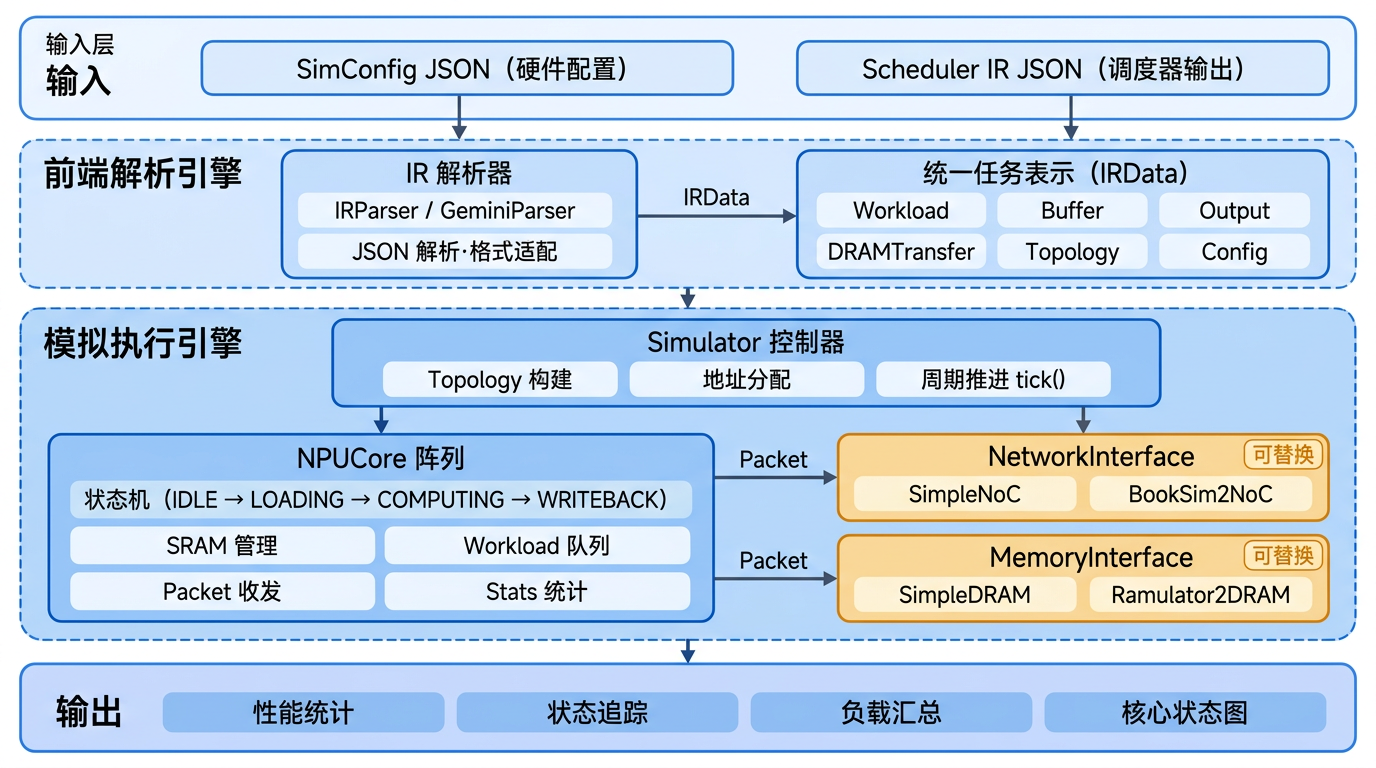
\includegraphics[width=1\linewidth]{Figures/c3_arch_overview.png}
  \caption{模拟器总体架构示意图}
  \label{fig:c3_arch_overview}
\end{figure}

上述模块切分背后有三项核心设计决策。（1）“IR 驱动”而非“踪迹驱动”。常见的加速器模拟器采用预先录制的访存或执行踪迹作为输入，适合在真实硬件上采样后离线重放。但对架构探索场景而言，每次修改映射或调度都需要重新录制踪迹，迭代成本高且难以在新架构上获得。本文以调度器直接生成的、带有显式依赖与数据流向的 IR 作为输入，使“改映射即改 IR”，在映射修改与参数扫描的场景下具有显著更低的迭代开销。（2）执行层不直接操作拓扑与地址。本文将拓扑解析（核心 ID 到 NoC 节点、DRAM 控制器路由）与地址分配（传输标识到物理地址）集中在引擎侧的辅助结构中，使计算核心只需以逻辑核心 ID 与传输标识为基本单位产生请求。这种分层有利于在后续支持更复杂的拓扑（如带 DRAM 控制器聚簇的非对称 Mesh）时，只需扩展拓扑与路由策略，而无需触动核心状态机。（3）NoC/DRAM 走抽象接口而非直接调用第三方应用程序接口（Application Programming Interface，API）。考虑到 BookSim2、Ramulator2 等第三方模拟器在调度粒度、时钟模型、完成通知机制上差异显著，本文在执行层与第三方模拟器之间引入统一的网络接口与存储接口，把差异封装在各自的封装器内部。这使得后续替换或新增子模块后端时，执行层逻辑完全不受影响。三项决策共同服务于同一目标：在保证端到端周期级精度的前提下，把映射改动架构参数改动与子模块后端改动三条迭代路径相互解耦。

\xsubsection{配置入口与拓扑构建}{Configuration Entry and Topology Construction}

用户通过命令行或配置文件指定 IR 路径与可选配置路径。配置为 JSON 格式，包含核心网格横/纵维度（可为 0 表示从 IR 补齐）、单核计算与 SRAM 参数、NoC 与 DRAM 参数（含后端类型、时钟比等）、拓扑（如 DRAM 控制器位置）及输出目录。用户可基于同一 IR、不同配置做对照实验。

模拟器在初始化阶段根据核心网格维度与可选的 DRAM 控制器位置列表构建 Mesh 拓扑。计算核心按行优先顺序放置在网格上，行索引 $i$、列索引 $j$ 的核心映射到 NoC 节点 $i \times W + j$（$W$ 为网格宽度）。当配置中给出 DRAM 控制器坐标时，控制器作为独立节点挂在 Mesh 边缘或角落（可在配置文件中选择不同策略），网格宽高自动扩展以容纳所有节点。此时 DRAM 请求需经 NoC 发往控制器节点，响应沿 NoC 返回，NoC 流量中同时包含核间通信与 DRAM 访存两类数据包。若未配置控制器位置，则 DRAM 走直连通道绕过 NoC，核间与 DRAM 流量完全隔离。拓扑构建完成后会执行合法性校验，确保计算核心与 DRAM 控制器不占用同一 NoC 节点，否则抛出异常终止。

本文模拟器选择 Mesh 作为默认 NoC 拓扑，主要基于三方面考量。其一是与工业实践对齐。当前主流多核神经网络芯片（如 Google TPU、NVDLA 多核版本以及国内若干多核神经网络芯片）在物理版图上普遍采用规则的二维 Mesh 或类似的片上网络。Mesh 拓扑能够直接对应到实际神经网络芯片的版图布局，模拟结果对工程研发具有参考价值。其二是路由规则简单且可解释。XY 路由等确定性路由在 Mesh 上无死锁、无活锁，路由结果可由核心坐标直接推导。这一性质便于在分析阶段手工核对核间通信路径，也便于结合核坐标与阶段占比进行热点归因。其三是与第三方 NoC 模拟器的兼容性。BookSim2 原生支持 Mesh 并以之为最成熟的测试拓扑，相关配置项与验证路径最为完善。对于 Torus、Fat-Tree、Dragonfly 等更复杂的拓扑，其对角径与带宽特性在超大规模系统中具有优势。然而在当前多核神经网络芯片的规模（数核至数十核）下，Mesh 的直径和平均跳数尚未成为系统瓶颈，且更复杂拓扑的引入会加大调度器侧映射策略的复杂度。因此，本文将 Mesh 作为默认实现，同时在拓扑模块中保留接口扩展点，便于后续研究中替换为其他拓扑。

当多个 DRAM 控制器挂在 NoC 上时，需要决定每次 DRAM 请求发往哪个控制器。模拟器支持三种路由策略。（1）最近节点策略：按发起请求的核心与各控制器之间的曼哈顿距离选择最近者，适合规则 Mesh 拓扑下减少平均跳数。（2）地址哈希策略：以请求携带的物理地址对控制器数取模，将不同地址段分散到不同控制器，提高多通道并行度。（3）轮转策略：按请求的全局发出顺序依次轮转到各控制器，实现请求级的负载均衡。策略由配置中的路由策略字段指定，默认为最近节点。上述拓扑与路由策略使核心 ID—NoC 节点—DRAM 控制器三者之间的映射透明化。引擎与核心仅按逻辑核心 ID 和传输标识操作，拓扑负责完成物理节点的翻译与路由决策。

拓扑确定了 DRAM 请求的路由路径，而请求中携带的物理地址则由地址分配器在加载 IR 后统一分配。分配器遍历 IR 中的 DRAM 读/写表以及各工作负载的输入缓冲与输出传输，收集所有涉及 DRAM 的传输标识及其数据大小。对同一传输标识在多处出现时取最大字节数，避免因多消费者引用导致的重复或不一致。随后按传输标识排序，依次为每条传输分配对齐到缓存行（默认 64 字节）的连续地址段。排序保证分配结果与传输标识的自然序一致，使地址空间布局确定且可复现。核心在发起 DRAM 读/写请求时，引擎根据传输标识查询分配器填入物理地址，供 Ramulator2 等后端按 Bank 与行进行时序建模。该分配策略的优势在于简单、确定且对齐良好，有利于 DRAM 后端的行缓冲命中率。后续可扩展为按张量维度的分区布局，以支持更复杂的地址映射研究。

\xsubsection{可配置的硬件与系统参数}{Configurable Hardware and System Parameters}

模拟器当前支持的配置维度如下：（1）核心规模与数据位宽：核心网格的横向与纵向维度、数据元素位宽。（2）单核计算与片上存储：MAC 单元数与向量单元数（分别用于 MAC 密集算子与向量/逐元素算子的周期估算）、SRAM 容量与读/写带宽，并可区分 PE（卷积/全连接）与向量处理器（Vector Processor，VP）（用于池化/逐元素操作）的带宽。（3）网络接口：最大未完成请求数、注入/弹出队列深度。（4）NoC：Flit 大小、跳数延迟与路由器延迟、后端类型（简化后端或 BookSim2）、时钟比、虚拟通道数与缓冲深度等。BookSim2 模式下还可指定外部配置文件路径。（5）DRAM：通道数、后端类型（简化后端或 Ramulator2）、时钟比、存储标准与组织（如 DDR4/HBM2）、时序与调度策略（如 FR-FCFS）、地址映射方式等。Ramulator2 模式下可指定外部文件配置。（6）拓扑：DRAM 控制器在 NoC 上的位置与路由策略（如最近节点策略）。上述参数均可通过 JSON 配置或命令行覆盖，便于在同一 IR 下进行设计空间探索与变量隔离实验。

\xsubsection{数据流、运行循环与统计输出}{Dataflow, Run Loop and Statistics}

模拟器内部根据 IR 格式创建解析器（当前支持 Gemini 格式），将 IR 解析为统一的任务数据，包含核心网格、每核工作负载列表、DRAM 读/写表等。若配置中未显式指定核心规模，则从解析结果中的核心网格横向与纵向维度补齐。若 IR 中带有调度器给出的 SRAM 容量需求，则据此自动调整每核 SRAM 容量约束。随后根据拓扑配置构建拓扑，用于将逻辑核心 ID 映射到 NoC 节点以及可选的 DRAM 控制器节点。地址分配器根据 IR 中的 DRAM 读/写表为每次传输分配物理地址，供后续 DRAM 请求携带。完成上述准备后，初始化核心：创建计算核心数组（每核绑定核心配置、SRAM 配置、网络接口配置与数据位宽），将各核工作负载列表按核注入各核心，并根据 NoC 与 DRAM 的后端类型分别实例化网络接口与存储接口（简化后端或 BookSim2/Ramulator2 封装）。

模拟器在所有核心均已完成为真前循环执行单周期推进并递增全局周期。单次推进的顺序为：（1）各计算核心按当前全局周期推进，产生待发送的 NoC 包或 DRAM 请求。（2）引擎从各核心收集发出的报文，根据目的节点是逻辑 DRAM 还是他核，分别注入存储接口或网络接口。若拓扑将 DRAM 挂在 NoC 上，则 DRAM 请求先封装为发往 DRAM 控制器节点的 NoC 包。（3）若有上一周期未注入的 DRAM 响应，则在本周期尝试注入 NoC。（4）推进 NoC 与 DRAM 一个周期。（5）从 NoC 按节点取回本周期到达的包并投递给对应核心或 DRAM 控制器。（6）从 DRAM 取回本周期完成的响应并投递给核心（或经 NoC 再投递）。该顺序保证先产生请求、再推进网络与存储、再投递响应，依赖满足与状态更新在时间轴上因果一致。模拟结束后统计总周期、总工作负载数、NoC 包数、DRAM 读写次数等，并可导出状态追踪与工作负载汇总表供后续分析使用。

模拟器运行结束后输出三类结果：（1）总周期、总工作负载数、NoC 注入/投递包数、DRAM 读/写请求与响应数。（2）每核统计信息，包括各核加载、计算、写回、NoC 背压停滞等阶段周期数，用于阶段分解与瓶颈归因。（3）启用踪迹选项时导出每核每周期状态序列与工作负载级起止周期汇总等文件。三类输出在后续分析中各有用处：第一类用于和硬件参考、解析模型对比总周期；第二类对应阶段占比分解，并可在多核下按核找出热点核；第三类用于排查异常时回放每核的状态序列，看清楚某段时间是卡在计算、加载、写回还是 NoC 背压。

\xsection{前端解析模块设计}{Front-end IR Parsing Module Design}\label{sec:c3_parse}

\xsubsection{调度器中间表示的定位}{Role of the Scheduler IR}

在展开解析器与格式细节之前，先明确本节所称 IR（Intermediate Representation，中间表示）在本模拟器中的含义与作用。本文中，IR 指调度器（或编译/映射工具链）输出的、描述已调度任务如何在多核神经网络芯片上执行的结构化数据。其内容通常包括：核心网格规模、各核上按依赖关系排列的工作负载列表、每项工作负载的算子类型与数据范围、核间与核—DRAM 之间的数据传输（含传输标识、源宿、大小等），以及可选的 SRAM 容量需求等。IR 不描述硬件微架构细节（如具体 NoC 路由、DRAM 时序）。它描述的是做什么、在哪做、依赖谁的逻辑视图。模拟器据此驱动周期级执行并统计性能。因此，IR 实质上是调度器与模拟器之间的接口约定。上游生成 IR，下游解析 IR 并转化为统一任务表示，二者通过 IR 的格式与语义解耦。

\xsubsection{解析器抽象与格式适配}{Parser Abstraction and Format Adaptation}

为避免执行层与具体 IR 格式强耦合，本文定义解析器抽象。对外仅暴露按路径解析并返回统一任务数据的接口。根据格式字符串可创建具体实现（当前支持 Gemini 格式）。后续若支持其他调度器输出格式，只需新增解析器并注册，模拟引擎与核心逻辑无需修改。

Gemini 解析器读入 JSON 根节点后，先读取全局字段：核心网格横向与纵向维度、批切分参数。若存在缓冲区容量，则判定为调度器 IR 并记录所需 SRAM 容量。除上述保留键外，专用键表示 DRAM 段，其下为 DRAM 读/写表。其余数字键表示核心 ID，对应值为该核上的工作负载数组。每个工作负载的解析包括：工作负载 ID、层名、层类型（或调度器 IR 中的 PE/VP/DT 等），映射为统一的算子类型（见下段）。再读取输出张量/权重等范围与尺寸、可选的解析周期。输入依赖数组解析为缓冲需求（每项包含传输标识、来源列表：来源类型、源核、大小、传输标识）。输出解析为输出传输（含传输标识与目的列表：目的类型、目的核、目的工作负载、层名）。调度器 IR 与汇编器 IR 在部分字段上存在位与字节的差异，解析器据此做换算，保证写入工作负载结构的尺寸为字节单位，供执行层与统计使用。

模拟器在统一任务表示中支持以下算子类型，算子类型与执行层计算时间估算及 SRAM 带宽选择一致。卷积与全连接为 MAC 密集型，计算时间按矩阵阵列算力的上界式估算，SRAM 使用 PE 带宽。池化如 MaxPool、AveragePool、GlobalAveragePool 按输出元素数与向量单元吞吐的上界估算，使用 VP 带宽。逐元素运算如 Add、Relu、Mul、Sub 等，同样按向量单元吞吐的上界估算，使用 VP 带宽。点对点传输对应数据搬运或 DT 类层，估算与带宽模型同逐元素。自定义在未显式匹配时归入此类，可按解析周期或默认规则估算。解析时由 IR 的层类型（如 Gemini 的 PE/VP/DT）与层名前缀（如 Conv、Gemm、MaxPool、Relu）映射为上述类型。计算时间估算的详细公式与可配置的 MAC 单元数/向量单元数见\,4.1.3\,节。

\xsubsection{后处理与统一任务表示}{Post-processing and Unified Task Representation}

解析完各核工作负载后，解析器执行三项后处理：（1）按依赖对每核内工作负载拓扑排序，保证消费某传输标识的工作负载排在产生该传输的工作负载之后。（2）根据各传输标识被引用的次数补全输出的引用计数，供核心在写回完成后做 SRAM 释放。（3）若调度器给出的核心 ID 非连续，则重映射为从 0 起的紧凑 ID，便于与核心数组下标一致。最终得到的统一任务数据包含核心网格规模、批切分、所需 SRAM 容量、各核工作负载列表、DRAM 读/写表。执行层仅依赖上述稳定数据结构，不直接依赖 JSON 键名。当上游 IR 格式演进时，仅需扩展或替换解析器实现，从而满足内容与形式分离的长期演进需求。

解析器产出的统一任务表示在内存中由两级结构组成。顶层的全局任务数据持有：核心网格维度、批切分参数、可选的全局 SRAM 容量需求、按核心 ID 索引的工作负载列表数组，以及 DRAM 读/写表（每条记录含传输标识、数据量、源/宿等，供地址分配与 DRAM 请求构造）。每个工作负载项包含：工作负载 ID、层名、算子类型、输入缓冲列表（每项含传输标识、来源类型与源核/DRAM、数据大小）、输出列表（每项含传输标识、目的列表与引用计数）、以及可选的解析周期或数据范围。执行层仅通过当前核的工作负载队列每项的缓冲需求与输出传输标识与引用计数驱动状态机与 SRAM 管理，不依赖 JSON 键名或具体字段命名。因此新增或调整 IR 格式时，只需在解析器内完成映射与单位换算，统一表示与执行层协议保持不变。

\xsubsection{中间表示与配置协同的语义对齐问题}{IR–Configuration Coordination and Typical Semantic Alignment Issues}

模拟器在加载 IR 后，部分配置项可由 IR 内容补齐或覆盖，以降低用户配置负担并保证与调度结果一致。例如，若配置中核心网格的横/纵维度为 0 或未给出，则从 IR 的网格维度补齐。若 IR 中带有调度器给出的缓冲区容量需求，且大于配置中的 SRAM 容量，则自动将每核 SRAM 容量上调至满足需求，避免因配置过小导致逻辑错误。反之，计算资源（如 MAC 单元数、向量单元数）、NoC/DRAM 后端类型与参数等仍以配置为准，便于在同一 IR 上扫描不同硬件参数进行设计空间探索。

尽管本节把解析器抽象得较为简洁，实际适配调度器 IR 的过程仍需处理若干语义层面的不一致问题，这些问题对于后续接入新的 IR 格式同样具有参考价值。第一，单位语义不一致：同一传输的数据量在调度器 IR 中可能以比特为单位、在汇编器 IR 中以字节为单位，也可能以张量元素个数给出。解析器需要结合数据位宽完成换算并统一到字节，否则 DRAM 地址分配与 SRAM 占用计算会出现系统性偏差。第二，算子类型命名空间不一致：调度器往往按其内部抽象（如 Gemini 的 PE/VP/DT）来标注工作负载，而执行层需要的是面向硬件的算子类型（卷积/全连接/池化/逐元素/点对点）以便选择对应的计算单元与 SRAM 带宽。解析器以层类型 + 层名前缀做联合映射，兼顾调度器自身类别与常见网络中的层命名惯例。第三，核心 ID 空间不紧凑：调度器为便于优化搜索，可能跳号或不使用全部核心（如仅在 2×2 子阵列上调度），解析器需在后处理中重映射为从 0 起的紧凑 ID，以便与核心数组下标一致并避免空索引。第四，传输引用计数的隐式依赖：同一输出传输可能被多个下游工作负载消费，而 IR 通常只显式给出消费者列表，解析器需据此推断引用计数，为后续引用计数归零后释放 SRAM 占用机制提供正确依据。这四类对齐工作封装在解析器内部，使得执行层与统一任务表示对 IR 格式的演进保持稳定，也为后续接入基于 MLIR 或自定义 JSON 的新 IR 格式提供了清晰的适配模板。

\xsection{面向对象的松耦合接口设计}{Object-oriented Loosely-coupled Interface Design}\label{sec:c3_iface}

\xsubsection{接口层的总体设计}{Overall Design of the Interface Layer}

网络接口与存储接口均以统一的报文结构为请求/响应单元，便于核间读请求与 DRAM 读/写请求共用同一数据形式。当拓扑将 DRAM 控制器挂在 NoC 上时，DRAM 流量可经 NoC 转发。采用抽象接口的核心动机在于：不同的子模块模拟器在请求粒度、数据表示、推进方式与完成通知机制上各不相同。例如 BookSim2 以 Flit 为最小调度粒度并由外部逐周期驱动，Ramulator2 则以缓存行为请求单元并通过异步回调通知完成。若执行层直接调用各模拟器的原生 API，则更换或新增后端时将牵连大量代码改动。通过在执行层与具体模拟器之间引入统一的接口层，将各模拟器的差异封装在接口实现内部，执行层仅依赖注入、推进与取回的抽象语义，从而在兼容现有模拟器的同时为接入其他 NoC 或 DRAM 模拟工具预留扩展空间。图\ref{fig:c3_loose_coupling_zh}从模块划分与可插拔后端的角度概括接口化松耦合架构带来的主要好处。

\begin{figure}[htbp]
  \centering
  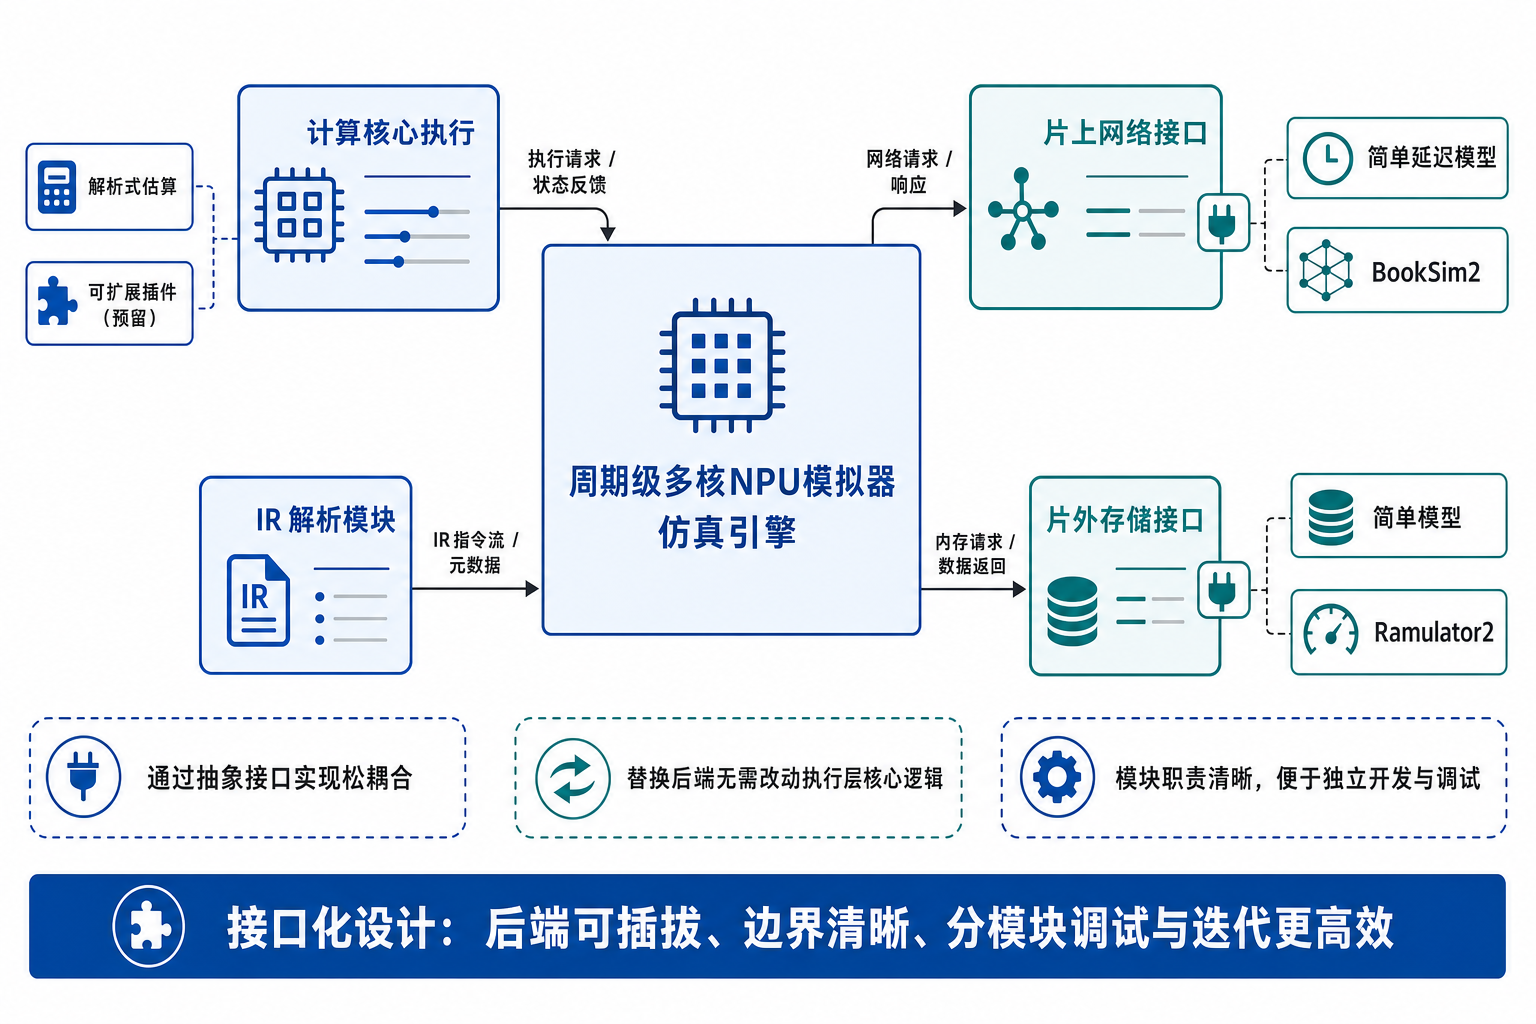
\includegraphics[width=0.95\linewidth]{Figures/loose_coupling_interfaces_zh.png}
  \caption{接口化松耦合架构示意图}
  \label{fig:c3_loose_coupling_zh}
\end{figure}

\xsubsection{拓扑与地址分配}{Topology and Address Allocation}

在将报文注入 NoC 或 DRAM 之前，模拟引擎依赖两类辅助结构。拓扑根据配置的核心网格与可选的 DRAM 控制器位置，将逻辑核心 ID 映射为 NoC 节点 ID，并确定 DRAM 请求应发往的控制器节点或直连存储接口。当 DRAM 控制器挂在 NoC 上时，拓扑还负责由核心到 DRAM 控制器的路径选择（如最近节点策略）。地址分配器在加载 IR 后根据 DRAM 读/写表为每条传输分配物理地址（按缓存行对齐）。核心在发起 DRAM 读/写请求时由引擎将对应地址填入报文，供存储接口与 Ramulator2 等后端使用。拓扑与地址分配使逻辑核心与传输标识与NoC 节点与 DRAM 地址解耦。接口层仅需按报文中的目的节点与地址转发。

\xsubsection{后端选择与报文生命周期}{Backend Selection and Packet Lifecycle}

NoC 与 DRAM 的具体实现由配置中的后端类型字段决定（可选简化后端、BookSim2 或 Ramulator2）。模拟引擎在初始化时通过工厂方法根据配置项创建对应的网络接口与存储接口实例。执行层仅持有抽象接口指针，不依赖具体后端类型。切换后端时仅需修改配置文件并重新运行，无需改动核心与引擎代码，从而实现两档精度与变量隔离。

报文从产生到被消费的路径可简述如下。核心在“加载”或“写回”阶段将待发送的读/写请求放入核内发送队列。引擎在每周期推进后遍历各核，收集本周期产生的报文，根据目的（他核或 DRAM）填入地址等信息后注入网络接口或存储接口。NoC/DRAM 在后续周期内推进。完成传输或访存后，本周期到达的响应由引擎按节点或目的核取回并投递到对应核心的接收入口。核心在下一周期推进开头处理到达的报文（写 SRAM、标记就绪、回复远端读请求等）。该数据流保证请求先于响应被处理、响应在后续周期对核心可见，与执行层所述的因果顺序一致。报文在生命周期的每一段都只走接口规定的入口和出口：核心通过发送队列把请求交给引擎，引擎通过注入接口把报文交给后端，后端把响应通过取回接口交回引擎，引擎再投递到核心。无论后端是简化模型还是 BookSim2/Ramulator2，所走的路径完全相同，差别只在路径中各段花掉的周期数。这样在排查问题时可以按段定位是核心、引擎、还是某一后端的行为不符合预期，也避免在替换后端时遗漏中间某一段的处理。

\xsubsection{统一报文类型与接口约定}{Unified Packet and Interface Contract}

报文信息包含：类型（读请求、读响应、写请求、写响应）、源/目的节点编号（目的为 DRAM 时使用保留编号）、传输标识、数据大小（字节）、DRAM 物理地址（由地址分配器分配）、注入周期/投递周期（用于简化后端与统计）。NoC 注入时可根据 flit 大小计算分片数（读请求仅头片，写请求为头片加载荷），供 BookSim2 等后端做分片传输。

网络接口提供的能力包括：按节点数与 NoC 配置初始化。注入报文并返回是否成功。每周期推进网络一次。按节点取回本周期到达的包。查询某节点是否可注入（背压判断）。查询当前周期。根据配置中的后端类型可选择简化后端或 BookSim2 封装。

存储接口提供的能力包括：按 DRAM 配置初始化。提交读/写请求并返回是否接受。每周期推进 DRAM 一次。取回本周期完成的响应包。可选地统计子请求总数。根据配置中的后端类型可选择简化后端或 Ramulator2 封装。

\xsubsection{网络接口}{Network Interface}

简化 NoC 后端不依赖外部 NoC 模拟库，按曼哈顿距离与配置的跳数延迟、路由器延迟计算端到端延迟。注入时记录投递周期并放入在途列表，每周期仅递增内部周期，到达时间已到的包在本周期取回。支持 NoC 与全局周期的时钟比，将 NoC 周期按比例折算到全局周期，便于与多时钟域实验一致。该模式无排队、无拥塞，适合快速回归与趋势对比。

模拟器封装第三方 BookSim2，在初始化时根据 NoC 配置生成或加载 BookSim2 配置文件（拓扑、虚拟通道数、缓冲深度、路由与分配延迟等），将逻辑节点 ID 映射为 BookSim2 子网与节点。注入时将报文转为 BookSim2 的 Flit 序列（头 flit 携带源/目的/传输标识/大小等元数据），按时钟比进行多速率推进。每周期查询各节点投递的 Flit，按报文编号重组为完整报文后返回。执行层仅调用网络接口的注入、推进与取回能力，不依赖文献\parencite{jiang2013booksim}所介绍的 BookSim2 的虚拟通道分配器、交换分配器等内部细节，从而实现松耦合与可替换性。

模拟器将 BookSim2 作为模拟器的 NoC 后端，需要解决报文与 Flit 序列之间的双向转换以及节点编号映射两类问题。

在报文到 Flit 序列的转换方面，模拟器内部以一个完整的报文为传输单元，而 BookSim2 以 Flit 为最小调度粒度。注入时封装器根据报文的数据大小与配置的 Flit 字节数计算所需 Flit 数。读请求通常仅携带元信息，映射为单个头 Flit。读响应与写请求则需在头 Flit 之后附加若干载荷 Flit。头 Flit 中编码源节点、目的节点、报文编号、传输标识与数据大小等元信息，供接收端在 Flit 到达后重组为完整报文。封装器为每个注入的报文分配递增的报文编号，并在内部维护报文编号到原始报文的映射表。

在 Flit 到报文的重组方面，BookSim2 在每周期按节点投递已到达的 Flit。封装器遍历所有目的节点，收集本周期到达的 Flit，并按头 Flit 中的报文编号进行聚合。当某报文编号对应的所有 Flit 均已到达时，从映射表中取出原始报文并标记投递周期，返回给引擎供后续核心消费。尾 Flit 的到达标志着该报文传输完成。这一机制使 BookSim2 内部的分片传输对执行层完全透明。

在节点编号与 Mesh 拓扑的对齐方面，模拟器的拓扑按核心网格 + 可选 DRAM 控制器节点构建 Mesh 拓扑网络，节点按行优先编号。BookSim2 的 Mesh 拓扑同样按行优先编号，但其节点数、宽度与高度需要与模拟器拓扑完全一致。封装器在初始化时将模拟器的 Mesh 宽度与高度写入 BookSim2 配置，并确保注入与投递时使用相同的节点 ID 空间，避免因编号偏移导致路由错误。多速率时钟桥接的具体机制（累加器与条件推进）将在跨时钟域同步部分详述。

\xsubsection{存储器接口}{Memory Interface}

简化 DRAM 后端固定读延迟与写延迟（如各 100 周期），提交请求时根据时钟比折算到全局周期，将响应放入在途列表并在投递周期到达时取回。无 Bank/行冲突、无排队，适合与高保真后端对照以隔离时序与调度的影响。

模拟器在初始化时根据 DRAM 配置加载或生成 Ramulator2 配置（通道数、Bank 组织、时序、调度策略等），并将报文的字节数与地址拆分为若干 cache-line 粒度子请求注入 Ramulator2 前端。Ramulator2 按自身时钟与时序推进，完成子请求后回调，封装器将同一传输标识的多个子请求聚合为一条读/写响应返回。支持 DRAM 时钟比，实现 DRAM 控制器与核心/NoC 的多速率推进。执行层仅通过存储接口的提交请求、推进与取回响应交互，不依赖文献\parencite{luo2023ramulator2}所介绍的 Ramulator2 的内部 API，从而保证松耦合。

与 BookSim2 类似，Ramulator2 的集成涉及请求粒度适配、异步回调聚合与地址语义对齐三方面。

在请求粒度适配方面，模拟器中的一次 DRAM 读或写对应 IR 中一个传输标识，数据量通常为数 KB 至数 MB。而 Ramulator2 的前端以缓存行（通常 64 字节）为请求粒度。封装器在提交请求时将报文的物理地址与字节数拆分为多个缓存行对齐的子请求，依次注入 Ramulator2 的请求队列。若某周期 Ramulator2 的请求队列已满，则剩余子请求在后续周期重试。封装器维护每个传输标识的已注入子请求数与已完成子请求数两个计数器。

在异步回调与响应聚合方面，Ramulator2 在内部完成某个子请求后通过回调通知封装器。封装器在回调中递增对应传输标识的已完成计数。当某传输标识的所有子请求均已完成时，封装器构造一条完整的读或写响应报文，放入可取回的完成队列。引擎在当前周期结束的取回响应阶段获取该报文并投递给对应核心。由此，多个缓存行级别的子请求对执行层表现为单次读/写操作的完成，简化了核心与引擎的逻辑。

在地址语义对齐方面，前文所述的地址分配器为每个传输标识分配了缓存行对齐的连续地址段。封装器在拆分子请求时从该基地址起按缓存行步进，生成的每个子请求地址落入 Ramulator2 的地址空间后经其内部的地址映射（通道、Bank 组、Bank、行与列）转化为具体的 DRAM 位置。不同传输标识的地址段互不重叠，避免了 Ramulator2 内部因地址冲突导致的非预期行缓冲行为。若配置中指定了多通道，地址的高位或低位交织可将不同传输的子请求分散到不同通道，提高并行度。

\xsubsection{接口化设计的意义}{Significance of Interface-based Design}

松耦合接口的意义体现在四点。（1）变量隔离：替换 NoC/DRAM 后端不改变模拟器推进逻辑与核心逻辑，对比简化后端与高保真后端时仅改配置项，减少混杂因素。（2）两档精度：可先用简化后端完成回归与趋势分析，再用 BookSim2/Ramulator2 给出拥塞与时序敏感的结论。（3）兼容异构子模块模拟器：不同第三方模拟器在请求粒度（Flit vs.\ 缓存行）、时钟模型（外部逐周期驱动 vs.\ 自身时钟推进）与完成通知方式（同步查询 vs.\ 异步回调）上差异显著。接口层将这些差异封装在各自的封装器实现内，使执行层无需关注后端是 BookSim2、Ramulator2 还是其他模拟工具，降低了集成新子模块模拟器的工程代价。（4）可扩展性：上述兼容机制也为后续引入新的 NoC 拓扑模型、DRAM 标准（如 HBM3、LPDDR5）或自定义统计插件提供了统一的扩展点，使设计空间探索具备持续演进能力。

在简化后端与高保真后端的适用场景方面，两种后端在精度与开销上各有侧重，便于按实验目的选择。简化后端无排队、无拥塞，延迟为距离或固定常数的理想化模型，运行快、结果可复现。该后端适合快速回归（如验证解析与状态机正确性）和趋势对比（如扫描核心数与 MAC 单元数时观察总周期随参数的大致走向），也可在与高保真后端对照时作为基线，以隔离仅因拥塞与时序所带来的差异。高保真后端则在周期级建模 NoC 的虚拟通道、仲裁与排队，并建模 DRAM 的 Bank/行缓冲与调度策略，能捕捉多核并发下的拥塞、背压与行冲突。该后端适合瓶颈归因（阶段分解与 NoC 背压停滞、存储等待占比），以及设计空间探索中需要区分计算墙、通信墙与存储墙时的定量分析。

在接口层支持的后续扩展方向上，上述网络接口与存储接口在抽象语义层面并未绑定具体的 NoC 拓扑或 DRAM 标准。因此本架构在不修改执行层的前提下，可以向多个方向自然扩展。在 NoC 侧，可以接入支持新型拓扑的模拟器（如 Garnet、FlooNoC 等），用以评估 Torus、Fat-Tree、层次化 Mesh 等更复杂拓扑在大规模多核神经网络芯片下的通信特性。在 DRAM 侧，接口仅要求注入读/写请求、每周期推进与取回完成响应的统一语义。因此 Ramulator2 之外的 DRAM 模拟器，以及 HBM3、HBM3E、LPDDR5 等更新的标准，只需在封装器内完成时钟比与地址分配的对齐即可接入。这种基于接口的可扩展性使本文模拟器不仅服务于本文的实验需求，也为后续围绕多核神经网络芯片的架构与系统研究提供了一个长期可演进的工程载体。



\xsection{高通用性计算核心建模}{General-purpose Core Modeling}\label{sec:c3_core}

\xsubsection{建模目标与抽象边界}{Modeling Goals and Abstraction Boundaries}

多核神经网络芯片端到端性能受计算、通信与存储共同影响。为在系统级研究中兼顾通用性与可解释性，本文以调度器 IR 中的工作负载为最小执行单元，对核心执行过程进行依赖驱动建模。核心在满足输入依赖后进入计算，计算完成后将输出写入本地 SRAM 并供其他核心拉取或写回 DRAM。该抽象能够覆盖 MAC 密集算子（卷积、全连接）与向量/逐元素算子（池化、激活等），并保留等待依赖到齐、注入队列满导致背压、写回 DRAM 拖尾等关键瓶颈形成机制，便于对端到端周期做阶段分解与归因。

从方法论上，本模拟器面向芯片早期设计阶段的架构参数与配置探索，以工作负载而非单条指令为最小建模粒度，这一取舍旨在可解释性与仿真成本之间取得平衡。指令级模拟能刻画更细的流水与调度行为，但多核、多工作负载场景下事件规模大，难以快速扫描配置。工作负载级抽象将调度器已决策的依赖与数据量作为输入，使端到端周期可归结为计算、加载、写回等阶段的叠加。由此便于回答瓶颈在计算、通信还是存储增加某类资源能否线性缩短时间等系统级问题，为架构探索与调度和硬件协同研究提供可操作的评估界面。而核内微架构与指令流水等细节被有意简化，以换取跨配置的快速扫描能力。这种粒度的选择有其适用范围：当研究问题涉及超标量发射、寄存器堆冲突等核内细节时，工作负载级建模会显得过粗，需要回到更精细的指令级或 RTL 级方法；但在本文关心的多核映射、片上互连与片外存储这一层，工作负载级粒度已经能够覆盖端到端周期中的主要影响因素。换言之，本节的建模并非希望取代指令级模拟，而是希望在前者过快、后者过慢的中间地带提供一个能用、能复现、能解释的评估手段。

单核在模拟中的职责边界为：维护当前工作负载队列与当前下标、按状态机推进、在加载阶段向 NoC/DRAM 发起读请求并消费到达的读响应、在写回阶段向 DRAM 发起写请求并等待写响应、响应他核对本核 SRAM 中已就绪数据的读请求。核心不直接调用 NoC/DRAM 的注入或发请求接口，而是将待发送的报文放入内部发送队列，由模拟引擎在每周期推进后统一从各核收集报文并注入网络或存储。到达的包由引擎按节点或目的核投递到各核的接收入口，核心在下一周期推进开头先处理本周期到达的报文。由此保证同一周期内先推进核心、再收集发送、再推进 NoC/DRAM、再投递的因果顺序。

\xsubsection{状态机设计}{State Machine Design}

本文将单核执行抽象为五态状态机：空闲（IDLE）、加载（LOADING）、计算（COMPUTING）、写回（WRITEBACK）、完成（DONE）。状态转移在单周期推进内按当前状态分支执行。

进入“空闲”状态后，若当前工作负载下标已达队列末尾，则转入“完成”并结束该核。否则取当前工作负载，根据其输入依赖中所有数据源的传输标识填入待加载集合。若待加载集合为空（无输入依赖），则直接转入“计算”并设置剩余计算周期。否则转入加载，等待依赖到齐。

在加载状态下，每周期尝试发起取数请求。对尚未请求过的传输标识，若已在本地 SRAM 且已就绪则从待加载集合移除。否则若来源为他核则构造发往该核的读请求，若来源为 DRAM 则构造发往 DRAM 的读请求，放入发送队列（若队列已满则统计因 NoC 背压停滞的周期数并本周期不再注入）。当所有缓冲已加载（即待加载集合为空）时，转入计算并设置剩余计算周期。

在计算状态下，每周期剩余计算周期减一。减至 0 时将当前工作负载的输出在 SRAM 中分配并标记为就绪（引用计数由 IR 后处理给出），并释放已消费的输入缓冲（对输入传输标识执行引用释放）。若存在输出目的为 DRAM，则转入写回并初始化待写回队列。否则当前工作负载完成，当前下标自增，回到空闲。

在写回状态下，每周期按 SRAM 读带宽从当前待写回块读取数据，凑满可发送的写请求后构造写请求（目的为 DRAM）放入发送队列，并将该传输标识加入待写回完成集合。当所有写请求已发出且写响应均已收回时，当前工作负载完成，回到空闲。

进入完成状态后，该核不再参与推进。

每周期推进内，在状态分支之前先执行以下操作。处理本周期投递来的包。将 NoC/DRAM 读响应数据按写带宽写入 SRAM 并标记就绪。对他核发来的读请求，若本核 SRAM 已就绪则回复读响应，否则继续挂起。图\ref{fig:c4_fsm} 给出状态机示意。
\begin{figure}[htbp]
  \centering
  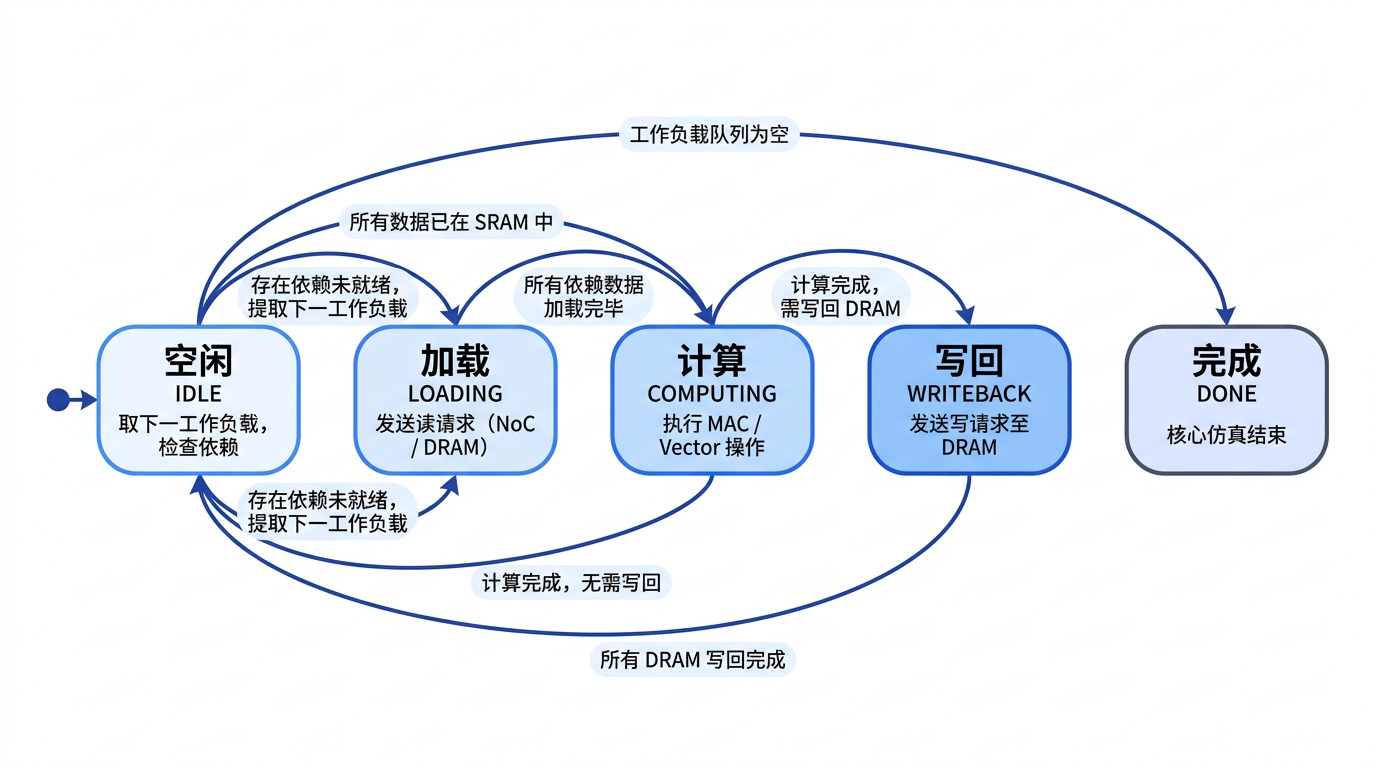
\includegraphics[width=0.95\linewidth]{Figures/c4_core_fsm_blue.png}
  \caption{核心五态状态机示意图}
  \label{fig:c4_fsm}
\end{figure}

\xsubsection{算子计算时间估算}{Operator Execution Time Estimation}

单个工作负载的计算周期由算子类型、张量尺寸与计算核心微架构三者共同决定。与精细的数据流仿真器不同，本模拟器面向芯片早期设计阶段的架构探索，核内采用上界式估算以换取跨配置扫描的速度与结果的可比性，不对流水填充、片上供数折损与分块对齐损失等微观效应做显式建模。

主流神经网络芯片的核内微架构在具体取舍上各异，但通常呈现出相似的功能组成。面向矩阵乘的规则阵列承担 MAC 密集计算，向量单元承担归约、逐元素与非线性计算，标量单元负责控制与地址生成。在此之外，核内通常配以由编译器/调度器显式管理的片上 SRAM，以及负责片内/片外数据搬运的 DMA 引擎。代表性设计包括文献\parencite{jouppi2017tpu}介绍的 Google TPU 矩阵单元（Matrix Unit，MXU）、文献\parencite{liao2019davinci,liao2021ascend}介绍的华为昇腾达芬奇立方单元（Da Vinci Cube Unit）、文献\parencite{veronesi2021nvdla}介绍的 NVDLA 卷积核心，以及文献\parencite{chen2016eyeriss}提出的 Eyeriss 脉动阵列等。本模拟器综合上述共性，在执行层将单个计算核心参数化为矩阵阵列、向量单元、片上缓存（容量与读写带宽可配）与数据搬运通路四部分。具体芯片在阵列拓扑、缓存层次与专用/共享策略上的差异，可通过参数扫描或子模块替换表达，但不作为核内精细建模的对象。

本模拟器按核内微架构的尺寸，对算子做朴素的数据流模拟：MAC 密集算子（卷积、全连接）按矩阵阵列每周期可做乘加计算的次数沿算子各维度逐块累积阵列占用周期。向量类算子（池化、逐元素等）按向量单元并行计算宽度的吞吐累积。数据搬运类工作负载按搬运带宽估算。当算子的张量维度与阵列或向量单元尺寸不整除时，按向上取整记入完整阵列周期，从而显式反映维度与阵列不对齐造成的尾效应。张量尺寸信息从 IR 中各工作负载的输出范围与权重尺寸字段解析获得，具体维度展开次序与分块策略不作为本文核内建模的对象。

该估算仅使用微架构的若干尺寸参数（矩阵 MAC 阵列尺寸、向量并行宽度、SRAM 容量与带宽等），不建模流水填充与排空、片上供数折损以及阵列内部利用率损失等二阶效应，属于计算时间的上界式估算。其结果在卷积主干等计算密集层上接近真实，但在小批量通用矩阵乘加、含归一化指数函数（Softmax）与层归一化（Layer Normalization, LayerNorm）等归一化的场景下时间偏小。片上缓存的供数约束不在本估算中体现，而是经由状态机的加载阶段按 SRAM 读写带宽与背压机制在系统级时间轴上计算，从而保证供数受限在端到端周期中仍可观测。

上述核内简化是面向早期架构探索的有意取舍：核内的分块策略、循环顺序、数据驻留方式以及流水填充等因素在同一算子上可带来数倍的执行周期差异，其精细建模本身是神经网络芯片研究中独立的课题\parencite{chen2016eyeriss,kwon2019maestro,parashar2019timeloop}。本模拟器将计算周期的产生过程实现为可替换的接口，与核心状态机、NoC/DRAM 推进等系统级推进逻辑解耦。后续可在不改动系统级仿真框架的前提下，将\,4.1.3\,节的上界式估算替换为含利用率折损、片上供数约束与流水填充的完整模型，或接入面向特定微架构的数据流仿真器（如文献\parencite{samajdar2020scalesim,kwon2019maestro,parashar2019timeloop}提出的 SCALE-Sim、MAESTRO、Timeloop 等），从而在保持系统级评估能力的前提下按需提升核内精度。

\xsubsection{片上内存管理}{Local SRAM Management}

本地 SRAM 以容量及其读写带宽为基本属性进行建模，容量以字节计，读写带宽以字节每周期计。在此之上，模拟器内部以传输标识为键维护 SRAM 条目，每项条目记录数据大小、数据类型、是否已就绪以及引用计数。其中数据类型可为输入特征、权重或输出特征，引用计数表示当前仍在引用该数据的消费者数量。分配时在容量允许下登记条目并累加已用容量。标记就绪将对应条目置为可消费。释放引用将引用计数减一，减至 0 时回收容量。这样，多消费者共享同一输出时，该输出在 SRAM 中保留至最后一个消费者释放引用，与第二章所述 IR 语义及解析器的引用计数后处理一致。

在 SRAM 拉取策略上，后文所述核间与 DRAM 的拉取式数据流，在网络与存储接口层面体现为消费者发起读请求、数据以读响应形式到达。在本地 SRAM 层面，本文采用与之衔接的到达后再占位、就绪后才可消费的策略，可概括为三点。（1）请求不等于已入 SRAM。核心在加载阶段发出读请求，仅表示向对端或 DRAM 索要数据，并不在本地预先为整块数据预留可消费条目。数据只有在读响应到达并被核心处理之后，才进入本地 SRAM 管理流程。（2）响应到达后的分配与写入。读响应到达时，仿真器先按当前工作负载对该输入的引用关系确定引用计数，并尝试为对应传输标识执行容量分配。若当前剩余容量不足，则将该响应暂存于重试队列，在后续周期中随其他数据释放或配置变化再次尝试分配，避免因瞬时峰值误判为永久失败。分配成功后，将本次加载的字节数记入待写入 SRAM 的剩余量，并在每个周期按有效写带宽（见下）消耗剩余量。当某传输标识对应的剩余量减至零时，将该条目标记为就绪，并从待加载集合中移除。由此，网络/存储侧完成传输与片上写入带宽填满本地 SRAM 并置就绪在时间上可分步刻画，便于区分远端延迟与片上写口瓶颈。（3）核间读对生产者 SRAM 的拉取。消费者向生产者发起的读请求，仅在生产者本地 SRAM 中该传输标识已就绪时立即回复读响应。否则请求挂起，待生产者侧计算完成并将输出写入本地 SRAM 并标记就绪后再回复。生产者侧在成功向消费者发送读响应时，按语义对相应条目做引用释放。这与（1）（2）共同构成谁消费、谁拉取、何时在本地变为可消费的闭环。

在带宽与类型分档上，有效写带宽与有效读带宽可根据当前工作负载类型在 PE 与 VP 两档配置间选取（例如卷积、全连接走 PE 档带宽，其余走 VP 档），与配置中统一写带宽字段并存。若将某档带宽配置为 0，则仿真器退化为当拍内完成整块逻辑写入并标记就绪，用于与带宽受限模式对照。每周期更新 SRAM 统计中的峰值占用，便于分析 SRAM 占用与映射可行性。峰值占用与引用计数语义的结合，使得某调度在给定 SRAM 容量下是否可行若缩小容量何处会成为瓶颈等问题可在仿真中直接观测，为映射与缓冲配置的可行性研究提供定量支撑。

\begin{figure}[htbp]
  \centering
  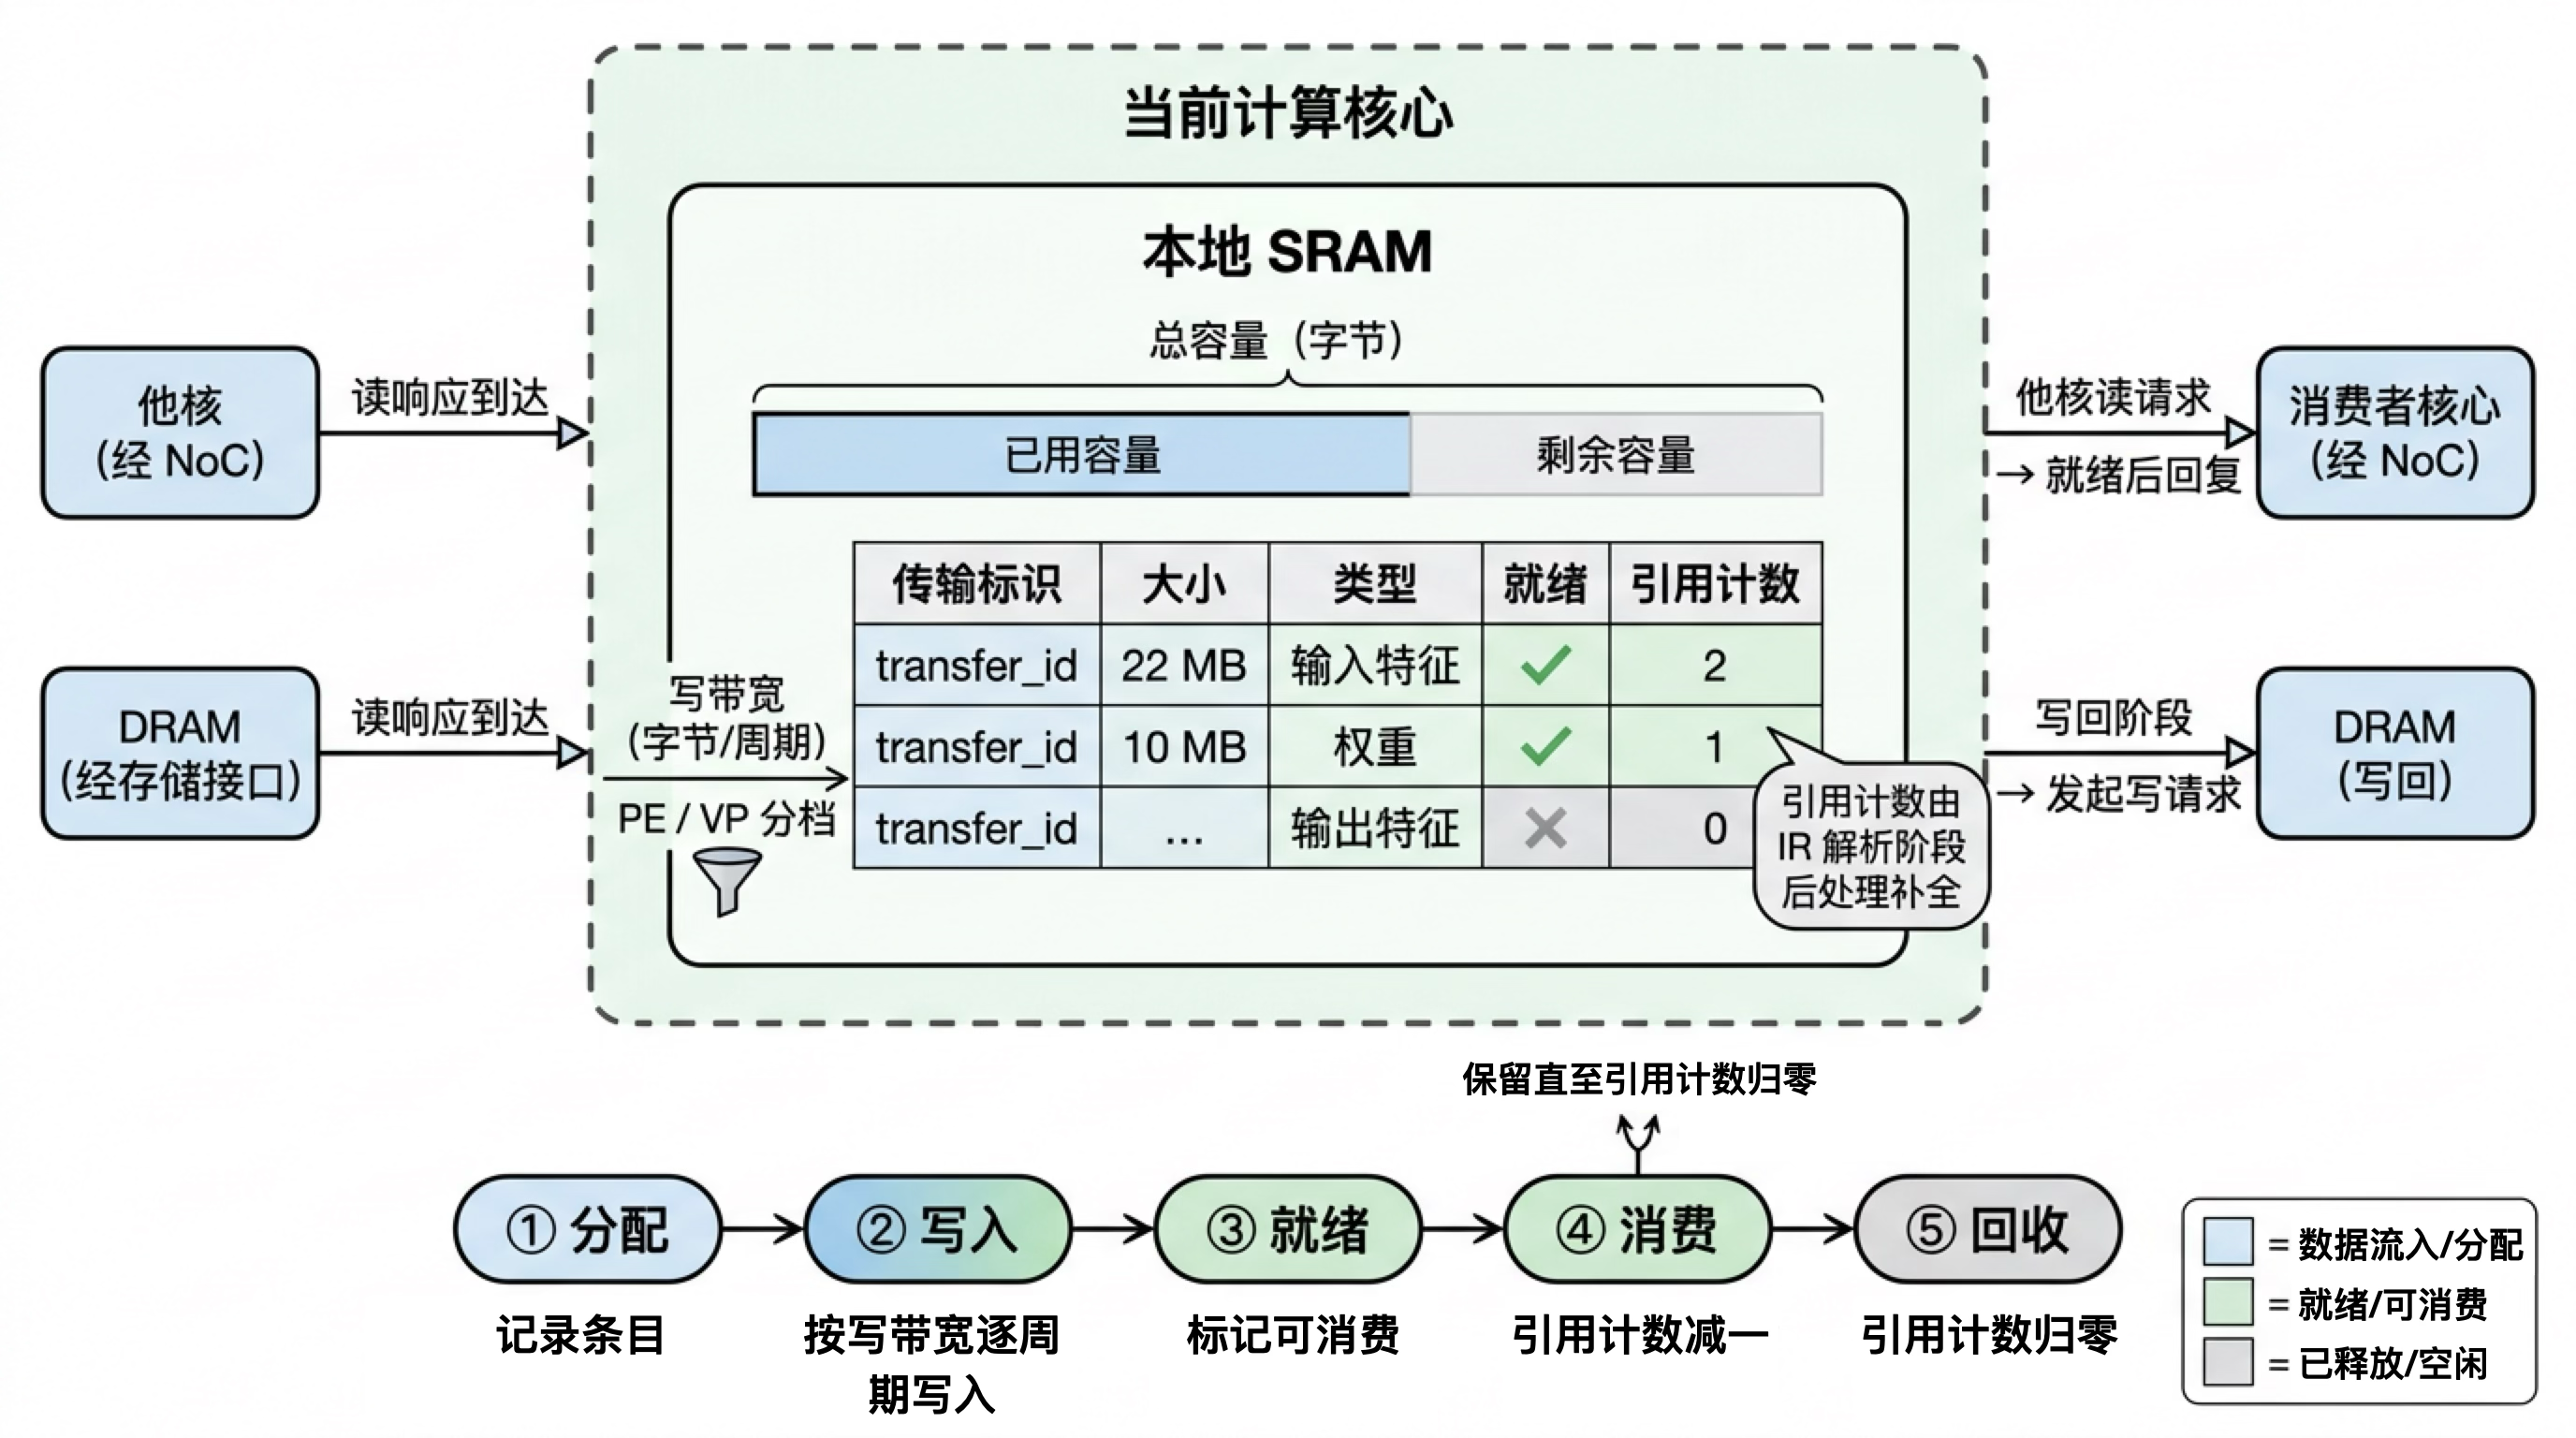
\includegraphics[width=0.95\linewidth]{Figures/sram_model.png}
  \caption{本地 SRAM 管理模型与数据生命周期示意图}
  \label{fig:c4_sram_model}
\end{figure}

图\ref{fig:c4_sram_model} 给出上述 SRAM 管理模型的整体结构与数据生命周期示意。左侧为数据来源（他核经 NoC、DRAM 经存储接口），中部为当前计算核心内的本地 SRAM 管理（包括容量分配、条目表与写带宽分档），右侧为数据去向（消费者核心经 NoC、DRAM 写回）。下方的生命周期流程展示了数据从分配、写入、就绪、消费到回收的完整过程，其中多消费者共享的数据在 SRAM 中保留至最后一个消费者释放引用。

\xsubsection{统计输出与可观测性}{Observables and Statistical Output}

执行层在每核、每周期上的行为最终体现为可导出的统计与踪迹，这些输出是连接设计与分析的桥梁。仿真结束后，每核可汇总得到在空闲、加载、计算、写回及因 NoC 背压停滞各阶段的周期数，以及完成的工作负载数、加载/写回的数据量、SRAM 峰值占用等。若开启状态追踪，还可按周期记录各核的状态转移序列（如从加载转入计算、从计算转入写回等），进而生成按核、按时间排列的阶段甘特图。上述统计与踪迹不改变仿真语义，但为端到端周期的阶段分解、瓶颈归因以及“热点核”识别提供了统一口径。后续实验将基于这些可观测量，对真实负载进行计算、访存与 NoC 背压的占比分解，并对多核场景下的工作负载时间线进行可视化，从而在系统级回答时间花在哪里哪些核或哪些阶段主导了总周期等问题。

\xsection{片上网络与内存子系统的集成机制}{Integration Mechanism of NoC and Memory Subsystem}\label{sec:c3_integration}

\xsubsection{拉取式数据流与接口集成}{Pull-based Dataflow and Interface Integration}

在模拟器中，核间数据采用拉取式（Pull-Based）数据流。消费者核心在加载阶段根据缓冲需求中的来源列表，向生产者核心（来源类型为他核时按源核 ID）或 DRAM（来源类型为 DRAM 时）发起读请求。生产者核心在处理到达报文时收到读请求。若本地 SRAM 中该传输标识已就绪，则构造读响应放入发送队列。否则将请求加入待回复的远端读请求列表，在后续周期中当数据就绪且发送队列未满时再回复。DRAM 读请求由引擎根据地址分配器填入物理地址后交给存储接口。写请求同样目的为 DRAM，由引擎注入 DRAM，DRAM 完成后再以写响应经引擎投递回核心，核心在处理到达报文时从待写回完成集合移除对应传输标识。所有报文均使用统一的报文结构（类型、源/目的、传输标识、数据大小、地址等），便于 NoC 与 DRAM 共用同一抽象。

在引擎侧的收集与投递流程中，各核心于单周期推进后，引擎遍历各核的待发送报文。若目的为 DRAM，则用地址分配器填入物理地址，再根据拓扑决定是经 NoC 发往 DRAM 控制器节点还是直接交给存储接口。若目的为他核，则必要时将源/目的转为 NoC 节点 ID 后注入网络接口。投递 NoC 包时按节点取回本周期到达的包并交给对应核心的接收入口（或交给 DRAM 控制器节点再转发给存储接口）。投递 DRAM 响应时从存储接口取回本周期完成的响应，根据目的投递给对应核心（若 DRAM 挂在 NoC 上，则响应先经 NoC 再在下一周期投递）。拓扑负责核心 ID 与 NoC 节点 ID 的映射、DRAM 控制器节点 ID 以及多控制器时的路由策略，从而支持仅计算核挂 NoC与NoC 上挂 DRAM 控制器两种部署方式。

% 在背压与队列约束方面，核心侧发送队列容量由网络接口配置限定。当队列满时，新发出的请求无法入队，本周期统计因 NoC 背压停滞的周期数，请求在下一周期重试。NoC 侧是否可注入在 BookSim2 封装中反映注入缓冲是否满，引擎可将无法注入的 DRAM 响应缓存在待注入队列并在后续周期重试注入，从而形成背压传递，使端到端周期能够反映拥塞与排队效应。

\xsubsection{多核并发与资源争用}{Multi-core Concurrency and Resource Contention}

对于数据流驱动的多核神经网络芯片，同一全局周期内多核并行推进，核间通信与共享资源的争用会直接影响端到端周期与瓶颈分布，仅讨论单核状态机不足以刻画系统行为。本小节说明多核并发在模拟中的体现、可能出现的竞态与争用现象，以及本文如何通过确定的推进顺序与资源建模来刻画并复现这些效应。

多核并发首先体现在单周期推进的组织方式上：引擎先对各核心依次执行一次推进，再从所有核心收集本周期发出的包并注入 NoC/DRAM。因此，每一全局周期内，多个核心可能同时处于加载（向不同生产者或 DRAM 发起读请求）、计算或写回。它们产生的请求在同一周期或相邻周期内集中进入 NoC 与 DRAM 的队列，形成对共享链路与存储资源的并发访问。依赖关系由 IR 中的传输标识与各核的待加载集合保证。消费者只有在收到对应读响应并标记就绪后才会离开加载，但何时收到取决于 NoC 的投递延迟与 DRAM 的排队与调度，二者均受多核并发流量影响。

在此基础上，模拟器可观察到若干典型的竞态与争用现象。（1）NoC 争用。多核同时向 NoC 注入时，同一链路或路由器上的多包需仲裁与排队。BookSim2 的虚拟通道分配、交换分配与路由延迟会随流量增大而放大尾延迟，部分核心的响应包可能因拥塞晚于理想延迟到达，从而拉长其加载阶段并统计到更多因 NoC 背压停滞周期。（2）DRAM 争用。多核的读/写请求进入同一 DRAM 控制器后，Bank/行缓冲与调度器（如 FR-FCFS）会引入排队与行冲突。Ramulator2 按时序与调度策略推进，同一周期内完成的响应数受通道与 Bank 并行度限制，部分请求的响应会延后完成，体现为消费者核心在加载或写回阶段等待更久。（3）生产者侧背压。当消费者向生产者发起读请求时，生产者需在数据就绪后回复读响应。若生产者本周期发送队列已满（因其他响应或本核写回占用），则无法注入该响应，请求在待回复的远端读请求中挂起，消费者端待加载集合无法清空，形成跨核的背压链。上述现象在真实多核数据流执行中均存在，本文通过多核每周期同时推进、统一收集注入以及 NoC/DRAM 周期级建模将其显式刻画为可观测的周期与阶段占比。

在确定性顺序与可复现性方面，模拟器内部不引入随机调度。同一周期内核心按数组下标顺序推进，收集报文按相同顺序遍历并注入，NoC/DRAM 的仲裁与调度由配置与请求到达顺序确定。因此，多核并发下的谁先被服务由确定的规则与数据依赖决定，不存在未定义的竞态。同一配置与同一 IR 下，总周期与各核各阶段占比可完全复现。争用与排队体现在同一资源被多核同时使用时，部分请求被延迟的客观结果上，而非模拟器实现的不确定性。

在死锁与核间同步问题上，拉取式数据流与有限发送队列的约束可能导致多核推进陷入死锁。若干核心均在加载或写回阶段等待来自他核或 DRAM 的响应，而对方因自身队列已满或尚未产生数据无法注入响应，形成相互等待、全局不再推进的局面。死锁的成因可从两方面理解。（1）依赖与资源环。若调度 IR 中存在跨核的依赖环（例如核心 A 的某工作负载依赖核心 B 的输出，核心 B 的某工作负载又依赖核心 A 的输出，且二者在时间上重叠或请求顺序导致互相阻塞），则在没有额外同步或请求排序约束时，可能出现A 等 B、B 等 A的循环等待。IR 本身描述的是数据依赖关系，调度器在生成 IR 时通常假定执行按某种顺序或缓冲容量充足，但并未在 IR 中显式编码防死锁的调度约束，因此 IR 在语义上并不保证无环或可运行性。（2）队列与背压的级联。当生产者核心的发送队列已满时，无法向消费者回复读响应，消费者会一直停留在加载并可能持续发起重试。若 NoC 或 DRAM 的注入侧也因背压无法接受新包，则请求与响应在多个节点上形成阻塞链，在极端情况下可能演变为系统级停滞。

\begin{figure}[htbp]
  \centering
  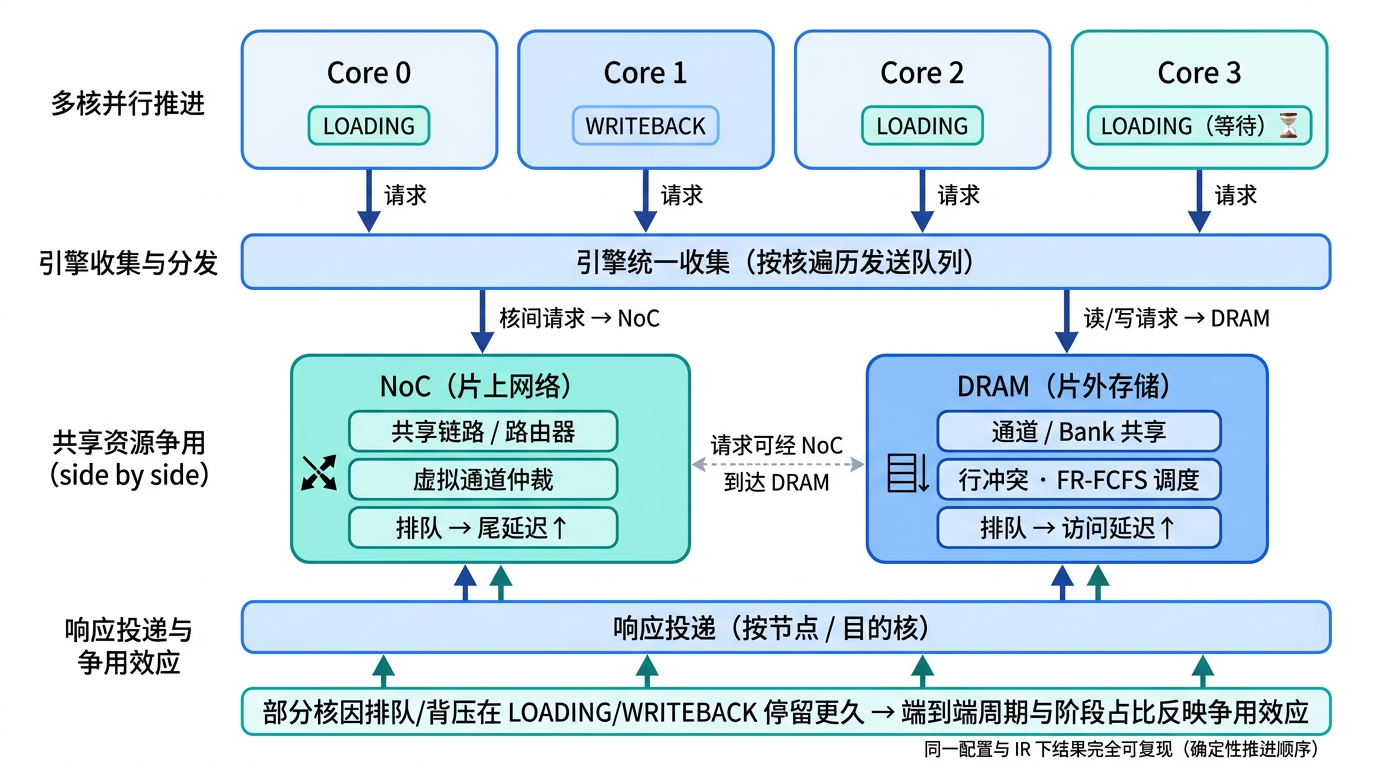
\includegraphics[width=\linewidth]{Figures/c4_concurrency_new.png}
  \caption{多核并发下请求汇聚与 NoC/DRAM 争用示意图}
  \label{fig:c4_concurrency}
\end{figure}

图\ref{fig:c4_concurrency} 给出多核并发下请求汇聚与资源争用的示意。多核在各自 LOADING 与 WRIT\allowbreak EBACK 阶段中产生的请求经引擎统一注入 NoC/DRAM。NoC 与 DRAM 在共享队列与仲裁下推进，响应再经投递回到各核。部分核心因排队或背压而在 LOADING 与 WRITEBACK 阶段上停留更久，从而在端到端周期与阶段分解中体现核间通信与共享资源的影响。争用与背压在模拟中并不依赖随机调度，而是由确定的推进顺序与请求到达顺序产生。因此因 NoC 背压而停滞的周期数、各核在加载/写回阶段的占比等指标均可稳定复现，可作为多核瓶颈分解与热点核分析的数据基础。当负载从单核扩展到多核时，非零的 NoC 背压占比与各核阶段分布的差异恰好可用于诊断通信瓶颈与热点核等设计问题。

\xsection{全局事件驱动与跨时钟域同步}{Global Event-driven and Cross-clock-domain Synchronization}\label{sec:c3_sync}

\xsubsection{跨时钟域模拟面临的问题}{Challenges in Cross-clock-domain Simulation}

首先是时间基准不统一。真实芯片中，计算核心、NoC 路由器与 DRAM 控制器往往由不同锁相环（Phase-Locked Loop，PLL）或时钟域驱动，三者频率可能为 \SI{1}{GHz} / \SI{500}{MHz} / \SI{266}{MHz} 等不同组合。若模拟器仅使用单一周期计数器且每拍让所有子系统各推进一周期，则等价于假设三者同频，无法区分DRAM 控制器更慢带来的排队与带宽折减。若改为为每个子系统维护独立时钟并异步推进，则事件顺序与谁先谁后的判定会变得复杂，且请求在核心周期 $t$发出、响应在DRAM 周期 $t'$完成时，需要明确 $t$ 与 $t'$ 的对应关系才能正确投递响应并统计端到端延迟。

其次是同步与修改可见性。请求在某一时刻注入 NoC 或 DRAM 后，响应应在该子系统已处理该请求并完成传输/访问之后才对核心可见。若子系统的“内部周期”与“全局周期”不一致，则必须约定响应何时被认为已完成，是以全局周期为刻度还是以子系统自身周期为刻度。若约定不当，可能出现响应在逻辑上早于请求被处理的因果错误，或同一全局周期内事件顺序依赖实现细节而难以复现。

最后，周期统计与带宽语义也可能存在分歧。端到端总周期通常以核心或系统主时钟为统计口径。当 DRAM 以较低频率运行时，其每 DRAM 周期处理能力不变，但每全局周期平均处理能力会按频率比下降。本模拟器在保持因果正确的前提下，让 DRAM 的等效带宽与每全局周期可完成的请求数随时钟比合理变化，以便扫描时钟比时观察到内存变慢导致端到端周期增加的预期趋势。

\xsubsection{跨时钟同步机制}{Cross-clock-domain Synchronization Mechanism}

本文采用单一全局周期 + 多速率推进的策略，在不动引擎调用顺序的前提下，让 NoC 与 DRAM 的等效频率可配置。

模拟器以全局周期计数器为唯一时间轴，所有何时发生的判定均以该周期为刻度。核心每全局周期推进一次。NoC 与 DRAM 的推进由引擎在每全局周期调用一次，但接口内部可根据时钟比决定本全局周期内子系统是否推进、以及推进几次。

在时钟比的语义上，配置项NoC 时钟比与DRAM 时钟比的约定为：时钟比 = 核心频率 / 子系统频率。因此时钟比 = 1 表示子系统与核心同频（每全局周期推进一周期）。时钟比 = 2 表示子系统以核心一半频率运行（每 2 个全局周期推进 1 周期）。时钟比 < 1 表示子系统频率高于核心（每全局周期可能推进多次，本项目通过累加器的累加与扣减实现）。这样，配置与真实核心 \SI{1}{GHz}、DRAM \SI{500}{MHz}的对应关系为 DRAM 时钟比 = 2，便于与数据手册或 RTL 时钟设定对齐。

各个模拟子系统各自维护一个累加器，每次被引擎调用时（即每全局周期一次）累加 1。当累加值不小于时钟比时，执行一次内部网络或存储的推进，并扣减时钟比（若时钟比大于 1，可用循环保证不漏推进）。因此，在任意一段全局周期数 $G$ 内，NoC/DRAM 的等效推进次数为 $G/\text{时钟比}$（取整由累加器自然体现）。既满足因果（请求先进入队列，随后仅在子系统推进时被处理），又使响应完成时间随时钟比增大而延后。

\xsubsection{时序示意与效果}{Timeline Illustration and Effects}

表\ref{tab:c4_cdc_timeline} 给出在 DRAM 时钟比为 2 时，连续若干全局周期内核心、NoC 与 DRAM 的推进关系。核心每全局周期推进一次。DRAM 仅在累加值达到时钟比时推进，因此第 1、3、5 拍才各推进一次，等效于每 2 个全局周期 1 个 DRAM 周期。请求在某一全局周期注入 DRAM 后，需等待 DRAM 内部经过若干次推进才会在取回响应时返回。由于 DRAM 推进频率降低，同一请求的从注入到响应可见的全局周期数会随时钟比增大而增加，从而在总周期与瓶颈分析中体现跨时钟域影响。

\begin{table}[htbp]
  \centering
  \caption{多速率推进示例表}
  \label{tab:c4_cdc_timeline}
  \small
  \begin{tabular*}{\textwidth}{@{\extracolsep{\fill}}cccccccccl}
    \toprule
    全局周期 $g$ & 0 & 1 & 2 & 3 & 4 & 5 & 6 & \ldots & 说明 \\
    \midrule
    Core 推进 & $\checkmark$ & $\checkmark$ & $\checkmark$ & $\checkmark$ & $\checkmark$ & $\checkmark$ & $\checkmark$ & & 每拍一次 \\
    NoC 推进（ratio=1） & $\checkmark$ & $\checkmark$ & $\checkmark$ & $\checkmark$ & $\checkmark$ & $\checkmark$ & $\checkmark$ & & 每拍一次 \\
    DRAM 推进（ratio=2） & -- & $\checkmark$ & -- & $\checkmark$ & -- & $\checkmark$ & -- & & 每 2 拍一次 \\
    累加器（DRAM） & 1 & 2$\to$0 & 1 & 2$\to$0 & 1 & 2$\to$0 & 1 & & 累加至 $\ge$2 则推进并扣减 \\
    \bottomrule
  \end{tabular*}
\end{table}

上述设计可达成以下效果：（1）因果一致。请求在某一全局周期被提交或注入后，仅在后续全局周期中、当子系统内部已推进并完成该请求时，响应才会在取回响应或按节点取回包时出现并投递给核心，不会出现响应早于请求。（2）可复现。同一配置与同一 IR 下，总周期与各阶段占比由确定的时钟比与累加器逻辑决定，无随机性或实现依赖。（3）可配置与可探索。通过将 DRAM（或 NoC）的时钟比设为大于 1，模拟器即可在不改动核心与引擎代码的前提下刻画内存/网络相对更慢的场景，本文实验也对此进行了参数扫描与敏感性分析。

\xsection{模拟器基本功能与精度验证}{Basic Functionality and Accuracy Validation}\label{sec:c3_accuracy}

\xsubsection{片上网络同步实验}{NoC Synchronization Experiment}\label{subsec:c3_mb1}

实验原理方面，本实验构造一个最小的双核、点对点（Peer-to-Peer，P2P）数据依赖场景，用于验证消费者核心必须等到生产者数据到达后才能开始计算的因果一致性。具体而言：第一个核心（Core\,0）作为生产者，先从片外存储器（DRAM）加载权重 \SI{32}{KB} 与输入特征 \SI{8}{KB}，接着进行 500 个模拟周期的计算，产生 \SI{128}{KB} 的输出并可供其他核心读取。第二个核心（Core\,1）作为消费者，需要先从 DRAM 加载自己的权重 \SI{64}{KB}，同时必须等待 Core\,0 产出的 \SI{128}{KB} 数据作为自己的输入特征，二者都就绪后再进行 300 周期计算，最后将结果写回 DRAM。若模拟器正确实现依赖传播，则 Core\,1 在加载阶段应一直等待，直到 Core\,0 的输出经核间通路到达后，才能结束加载、进入计算阶段。

实验过程上，硬件与负载配置如下。硬件配置：双核拓扑。NoC 与 DRAM 分别采用前文定义的 高保真后端（BookSim2 + Ramulator2，完整建模 DDR 时序与网络排队）与 简化后端（固定延迟、简化建模）各运行一次，以对比两种后端下核间依赖与访存延迟的叠加效果。运行负载：即上述Core\,0 生产者、Core\,1 消费者的两层调度，输入与权重规模如上。实验时对两种后端分别执行模拟，并开启状态记录。从模拟得到的状态时间线中读取每个核心在加载、计算、写回各阶段的起始与结束周期，以及各阶段持续时长，用于填表与绘图。

实验结果方面，表\ref{tab:mb1}给出两种后端下各核的状态转移时间点与阶段时长。

\begin{table}[H]
  \centering
  \caption{片上网络同步实验结果}
  \label{tab:mb1}
  \small
  \begin{tabular*}{\textwidth}{@{\extracolsep{\fill}}llrrr}
    \toprule
    后端 & 核/阶段 & 起始周期 & 结束周期 & 时长 \\
    \midrule
    \multirow{5}{*}{高保真后端} & Core\,0 LOADING  & 0    & 207  & 207 \\
                                    & Core\,0 COMPUTING & 207  & 707  & 500 \\
                                    & Core\,1 LOADING  & 0    & 2000 & 2000 \\
                                    & Core\,1 COMPUTING & 2000 & 2300 & 300 \\
                                    & Core\,1 WRITEBACK & 2300 & 2456 & 156 \\
    \cmidrule{2-5}
                                    & 总周期 & \multicolumn{3}{r}{2458} \\
    \midrule
    \multirow{5}{*}{简化后端} & Core\,0 LOADING  & 0   & 180 & 180 \\
                             & Core\,0 COMPUTING & 180 & 680 & 500 \\
                             & Core\,1 LOADING  & 0   & 938 & 938 \\
                             & Core\,1 COMPUTING & 938 & 1238 & 300 \\
                             & Core\,1 WRITEBACK & 1238 & 1402 & 164 \\
    \cmidrule{2-5}
                             & 总周期 & \multicolumn{3}{r}{1404} \\
    \bottomrule
  \end{tabular*}
\end{table}

图\ref{fig:c5_mb1_trace}根据高保真后端运行得到的状态转移踪迹绘制，横轴为模拟周期（Cycle），纵轴为两核（上方为 Core\,1，下方为 Core\,0），图中颜色表示各核所处状态：橙色为 LOADING，蓝色为 COMPUTING，红色为 WRITEBACK。该图直观展示两核的状态转移时间线：Core\,0 先完成 LOADING 与 COMPUTING，Core\,1 在长时间 LOADING（等待 Core\,0 的输出与 DRAM 响应）后才进入 COMPUTING 与 WRITEBACK，与表\ref{tab:mb1}一致。

对结果的分析如下：（1）因果一致性验证通过。两种后端下，Core\,1 均在 Core\,0 完成计算（高保真后端下约 707 周期，简化后端下约 680 周期）之后才结束加载阶段、进入计算阶段（高保真后端下 Core\,1 加载约 2000 周期，简化后端下约 938 周期），说明依赖传播的因果约束被正确执行。模拟输出的状态记录也显示，Core\,1 在加载阶段明确标记为等待来自 Core\,0 的 \SI{128}{KB} 数据，与上述依赖关系一致。（2）计算时长一致。两种后端下 Core\,0 与 Core\,1 的计算阶段分别为 500 与 300 周期，与调度中设定的计算量完全吻合，验证了计算建模的正确性。（3）DRAM 后端影响访存阶段。高保真后端下 Core\,1 的 LOADING 阶段为 2000 周期，简化后端下仅为 938 周期。差异来自 Ramulator2 的 DDR4 时序约束（tRCD、tCL 等）使 DRAM 响应延迟更高，同时 Core\,1 还需等待 Core\,0 的计算及 NoC 传输完成，两者串行叠加导致 LOADING 时间显著拉长。（4）NoC 数据包一致。两种后端均产生 2 个 NoC 数据包（从 Core\,0 到 Core\,1 的请求与响应），验证了核间通信路径的正确性。

\begin{figure}[H]
  \centering
  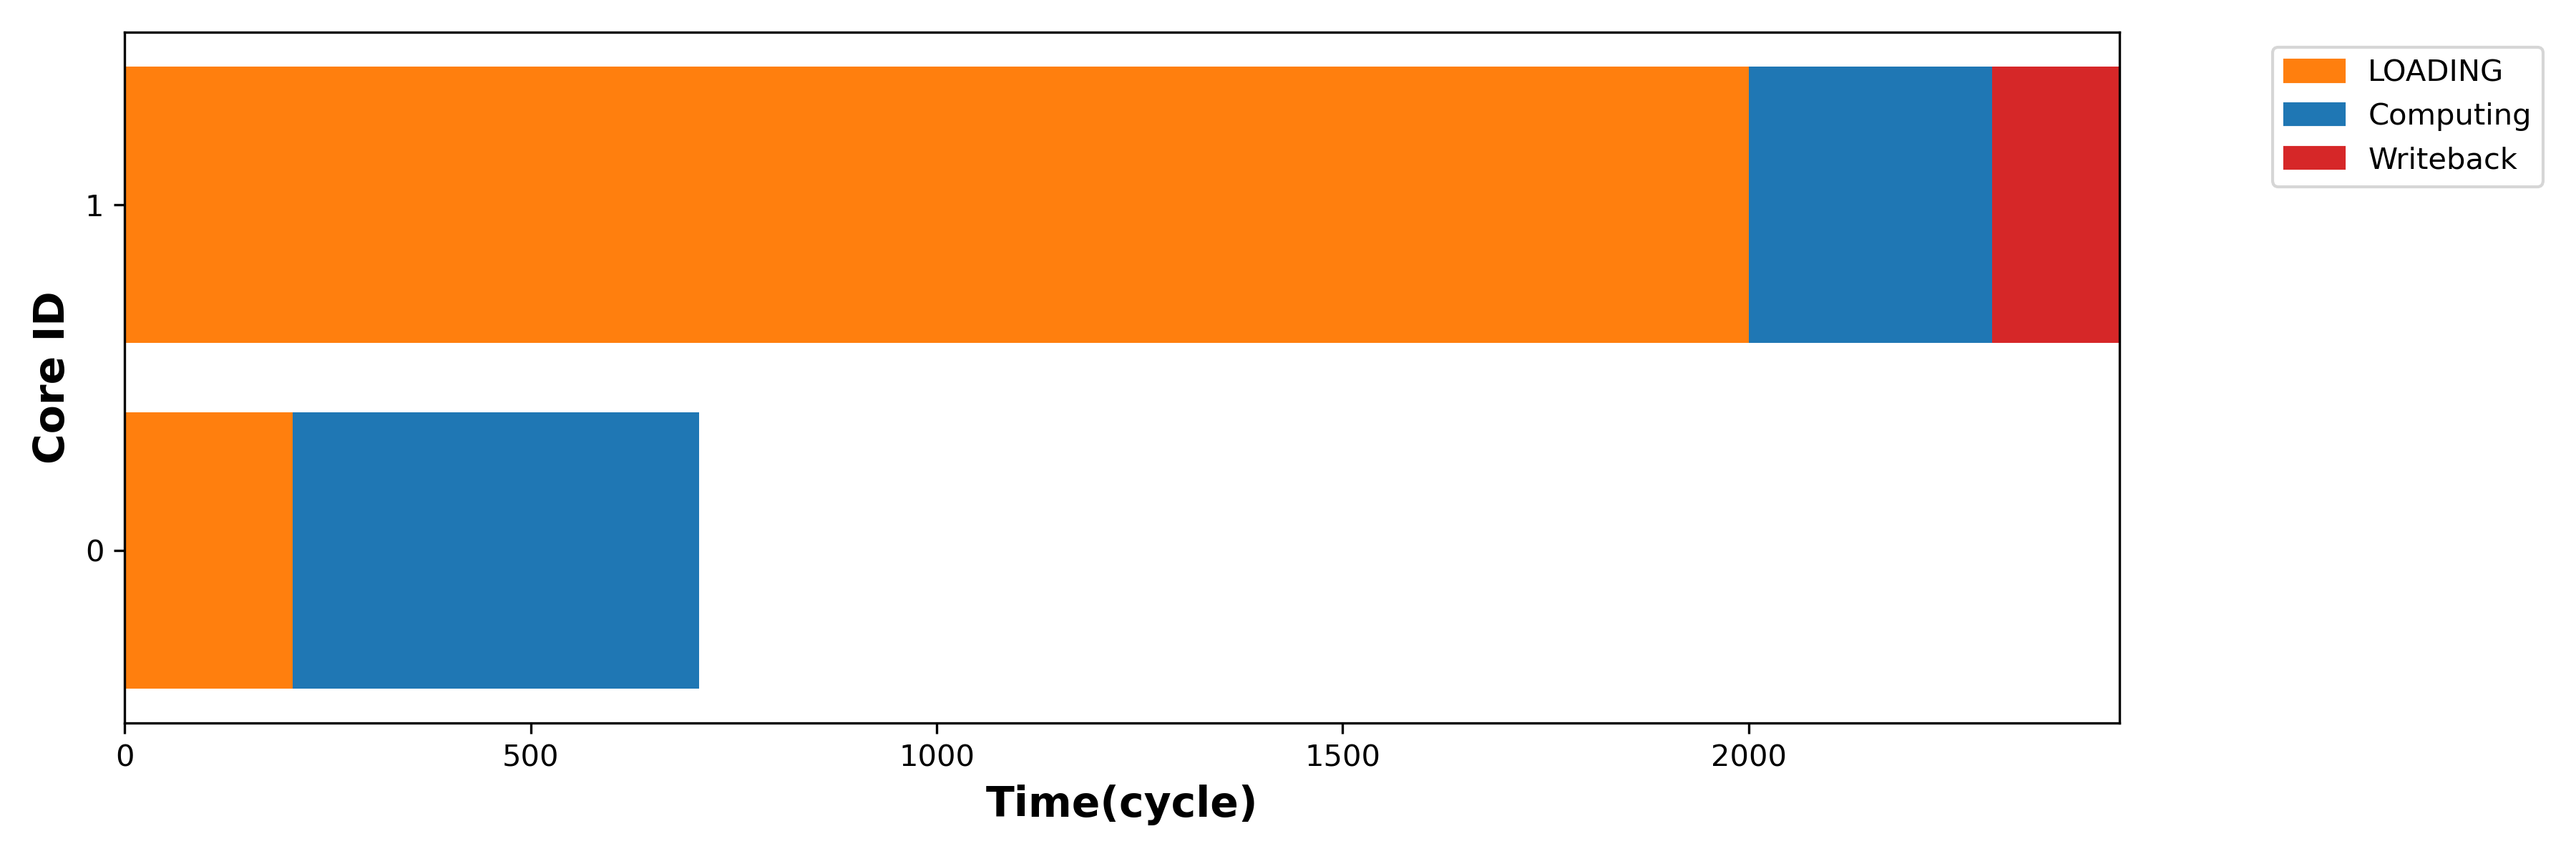
\includegraphics[width=0.78\linewidth]{Figures/c5_mb1_trace.png}
  \caption{片上网络同步实验高保真后端状态转移时间线}
  \label{fig:c5_mb1_trace}
\end{figure}

\xsubsection{内存同步实验}{Memory Synchronization Experiment}

实验原理方面，本实验在单核上执行两层串行计算，且两层所需的输入与权重全部来自片外存储器（DRAM），不涉及核间数据传递，用于验证：（1）单核、仅 DRAM 依赖时，不应产生任何 NoC 数据包。（2）简化后端与高保真后端两种后端在纯 DRAM 访存场景下的周期差异，量化 DDR 时序建模对访存阶段的影响。具体负载为：第一层从 DRAM 加载权重 \SI{32}{KB} 与输入特征 \SI{8}{KB}，计算 500 周期后向 DRAM 写回 \SI{128}{KB}。第二层从 DRAM 加载权重 \SI{64}{KB} 与输入特征 \SI{128}{KB}（即第一层写回的数据），计算 300 周期后向 DRAM 写回 \SI{32}{KB}。两层的计算量固定，差异仅体现在 DRAM 的加载与写回阶段上。

实验过程上，硬件配置为单核拓扑，NoC 与 DRAM 仍分别采用 高保真后端与 简化后端各运行一次。运行负载即上述两层、仅 DRAM 依赖的调度，无核间通信。对两种后端分别执行模拟并记录状态时间线，从时间线中读取每一层在加载、计算、写回各阶段的起止周期与时长，用于填表与对比。

实验结果方面，两种后端下各层的执行时间线见表\ref{tab:mb2}。

对结果的分析如下：（1）NoC 数据包为 0。两种后端下均无 NoC 流量（DRAM 直连核，未经过 NoC），验证了单核 DRAM-only 场景下通信路径的正确性。（2）计算时长一致。Layer1 与 Layer2 的 COMPUTING 阶段在两种后端下分别为 500 与 300 周期，与调度中给定的计算周期一致。（3）DRAM 模型差异集中在访存阶段。高保真后端下，Layer1 的 WRITEBACK 为 651 周期（简化后端 356，增幅 83\%），Layer2 的 LOADING 为 853 周期（简化后端 484，增幅 76\%）。这反映了 Ramulator2 的 DDR4 时序（行激活、列读取、Bank 冲突、请求排队）对大块数据传输的影响：Layer1 写回 \SI{128}{KB}、Layer2 加载 \SI{192}{KB}（64+128），数据量越大时 DDR 时序约束越显著。（4）总周期差异。高保真后端总周期 2685，简化后端为 1987，高保真后端高出 35\%。差异完全来自 DRAM 访存阶段，计算阶段无差异。后续 ZeBu 对比实验统一采用高保真后端，以在包含完整 DDR 时序建模的条件下评估模拟器的端到端精度。

\begin{table}[H]
  \centering
  \caption{内存同步实验结果}
  \label{tab:mb2}
  \small
  \begin{tabular*}{\textwidth}{@{\extracolsep{\fill}}llrrr}
    \toprule
    后端 & 层/阶段 & 起始周期 & 结束周期 & 时长 \\
    \midrule
    \multirow{7}{*}{高保真后端} & Layer1 LOADING    & 0    & 207  & 207 \\
                                    & Layer1 COMPUTING  & 207  & 707  & 500 \\
                                    & Layer1 WRITEBACK  & 707  & 1358 & 651 \\
                                    & Layer2 LOADING    & 1359 & 2212 & 853 \\
                                    & Layer2 COMPUTING  & 2212 & 2512 & 300 \\
                                    & Layer2 WRITEBACK  & 2512 & 2683 & 171 \\
    \cmidrule{2-5}
                                    & 总周期 & \multicolumn{3}{r}{2685} \\
    \midrule
    \multirow{7}{*}{简化后端} & Layer1 LOADING    & 0    & 180  & 180 \\
                             & Layer1 COMPUTING  & 180  & 680  & 500 \\
                             & Layer1 WRITEBACK  & 680  & 1036 & 356 \\
                             & Layer2 LOADING    & 1037 & 1521 & 484 \\
                             & Layer2 COMPUTING  & 1521 & 1821 & 300 \\
                             & Layer2 WRITEBACK  & 1821 & 1985 & 164 \\
    \cmidrule{2-5}
                             & 总周期 & \multicolumn{3}{r}{1987} \\
    \bottomrule
  \end{tabular*}
\end{table}

两个微基准验证了模拟器三项基本能力：核间依赖因果一致性（片上网络同步实验）、DRAM 闭环正确性（内存同步实验）、以及简化后端/高保真后端在计算阶段完全一致而在访存阶段体现 DDR 时序差异。这为后续统一采用 高保真后端进行 ZeBu 精度校验与多核设计空间探索奠定了基础。

\xsubsection{精度验证实验}{Accuracy Validation Experiment}
\label{subsec:c5_zebu}

实验原理方面，Synopsys ZeBu硬件模拟平台在单核配置下执行与本模拟器相同的调度IR所生成的汇编指令，并通过硬件踪迹记录每条指令的执行区间$[\mathit{start},\mathit{end}]$。以ZeBu全程序总周期（$\max(\mathit{end})$）作为基准，与本模拟器的总时钟周期对比。为使精度评估涵盖完整的系统级时序（包括 DDR 行列时序与请求排队），本实验采用高保真后端（BookSim2 + Ramulator2）与 ZeBu 硬件模拟对照。

实验过程上，ZeBu 侧的总周期取自 Gemini-Compiler-IR 项目发布的单核预跑结果。本实验在模拟器一侧采用单核、高保真后端配置（BookSim2 + Ramulator2），选取 ResNet34 与 ResNet50 在批大小 1 与 4 下的调度结果分别运行模拟并记录总周期，与上述 ZeBu 参考周期逐项对比。

实验结果方面，表\ref{tab:zebu_validation}给出上述四种配置下模拟器与 ZeBu 的总周期及相对误差。

\begin{table}[H]
  \centering
  \caption{与 ZeBu 硬件模拟的总周期对比表}
  \label{tab:zebu_validation}
  \small
  \begin{tabular*}{\textwidth}{@{\extracolsep{\fill}}lrrrr}
    \toprule
    模型 & 批大小 & ZeBu周期 & 模拟器周期 & 相对误差（\%） \\
    \midrule
    ResNet34 & 1  & 1,922,067 & 1,890,695 & $-$1.63 \\
    ResNet34 & 4  & 4,280,215 & 4,501,725 & +5.18 \\
    ResNet50 & 1  & 2,545,655 & 2,432,592 & $-$4.44 \\
    ResNet50 & 4  & 5,470,662 & 5,653,354 & +3.34 \\
    \bottomrule
  \end{tabular*}
\end{table}

对结果的分析如下：（1）误差均在 $\pm$5.2\% 以内。4 种配置的相对误差范围为 $-$4.44\% 至 +5.18\%，说明在包含完整 DRAM 时序建模的条件下，模拟器与 ZeBu 硬件模拟在总周期上吻合良好。（2）正负偏差并存，无系统性偏移。批大小为 1 时模拟器周期略低于 ZeBu（$-$1.63\%、$-$4.44\%），批大小为 4 时略高（+5.18\%、+3.34\%）。偏差方向与批大小有关：批较小时 Ramulator2 的 DDR 时序对小规模访存的建模与 ZeBu 存在微小差异。批增大后，工作负载级阶段划分与 ZeBu 指令级执行在访存重叠上的建模粒度差异被放大。（3）趋势一致。随批大小从 1 增至 4，两个模型的总周期均近似线性增长（ResNet34 由 1.89M 增至 4.50M，对应 ZeBu 由 1.92M 增至 4.28M。ResNet50 由 2.43M 增至 5.65M，对应 ZeBu 由 2.55M 增至 5.47M），趋势一致。

\xsubsection{实验结论}{Experimental Conclusions}

综合片上网络同步实验、内存同步实验与模拟器精度验证实验三组实验，本节得到以下结论。片上网络同步实验验证了模拟器在双核点对点依赖下的因果一致性，状态机在等待数据后进入计算的行为符合预期。内存同步实验通过 简化后端与高保真后端在不同并发度下的对比，印证了可插拔后端在快速校验与高保真评估间的不同定位。在单核、调度一致、统一采用 高保真后端（BookSim2 + Ramulator2，包含完整 DDR 行列时序与请求排队）的配置下，本模拟器与 ZeBu 硬件模拟平台在 4 种 ResNet 配置上的总周期相对误差均控制在 $\pm$5.2\% 以内，验证了端到端时序模型的准确性。三组实验共同表明，本模拟器具备可信的建模能力，为后续多核瓶颈分析与设计空间探索提供了可靠基础。


\xsection{本章小结}{Chapter Summary}

本章完成了多核神经网络芯片周期级模拟器的设计、实现与精度验证。从问题出发，本章先把映射、互连与存储这三层耦合作为模拟器需要同时承载的对象，并据此提出 IR 直驱、统一任务抽象与多速率周期级一致三项设计目标。在此基础上，本章给出了由配置入口、前端解析、执行引擎、接口层与统计输出构成的整体架构，并为 NoC 与 DRAM 设计了抽象接口与对应的简化、高保真两种后端，使后端的替换不会影响执行层的语义。执行层方面，本章用五态状态机刻画了核内依赖到齐、加载、计算与写回的推进过程，并把拉取式数据流、统一报文与多核并发下的资源争用统一纳入按周期推进的模型。同步机制方面，本章以全局周期为唯一时间基准，通过时钟比让 NoC 与 DRAM 控制器即便频率不同也能保持因果一致与可复现。精度方面，本章设计了片上网络同步、内存同步与 ZeBu 对照三组实验，分别用于检验因果与时序的正确性、DRAM 闭环时序的一致性，以及在真实负载上与硬件参考的总周期一致性。本章建立的模拟平台与精度结论，是下一章开展瓶颈归因与设计空间探索的工程基础。
